%\documentclass[envcountsect,11pt,trans]{beamer}
\documentclass[11pt,aspectratio=169]{beamer}
\usepackage[english]{babel}
\usepackage[ansinew]{inputenc}
\usepackage{times}
\usepackage{xcolor}
\usepackage{graphicx}
\usepackage{rotating}
\usepackage{bbding,pifont} % two dingbat fonts
\usepackage{amsmath}
\usepackage{amsfonts}
\usepackage{amssymb}
\usepackage{fancybox}
\usepackage{epstopdf}
\usepackage{eso-pic}
%\usepackage[round]{natbib}
\usepackage{ngerman}
\usepackage{tcolorbox}
\usepackage{colortbl}
%\usepackage[authordate,bibencoding=auto,strict,backend=biber]{biblatex-chicago}
%\usepackage{natbib}
%\usepackage[style=bath, backend=biber]{biblatex}
\usepackage{ulem}
\usepackage{tikz}
\usepackage{booktabs}
\usepackage{longtable}
\usepackage{hyperref}
\usepackage{array}
\usepackage{appendixnumberbeamer}
\usepackage[T1]{fontenc}
\usepackage{adjustbox}
\usepackage{listings}
\usepackage{uarial}
\usepackage{fancyvrb}
\usepackage{subfigure}
\renewcommand{\familydefault}{\sfdefault}

\newcommand*\circled[1]{\tikz[baseline=(char.base)]{
            \node[shape=circle,draw,inner sep=2pt] (char) {#1};}}
\newcommand{\E}{\operatorname{E}}
\newcommand{\Var}{\operatorname{Var}}
\newcommand{\overbar}[1]{\mkern 1.5mu\overline{\mkern-1.5mu#1\mkern-1.5mu}\mkern 1.5mu}
\DeclareMathOperator*{\argmin}{arg\,min}
\DeclareMathOperator*{\argmax}{arg\,max}
% \use\smallpackage{pgfpages}
% \pgfpagesuselayout{4 on 1}[a4paper,border shrink=10mm,landscape]

%\xdefinecolor{MyColor}{rgb}{0.14,0.17,0.52}
%\xdefinecolor{MyColor}{rgb}{0.29,0.53,0.82}
%\xdefinecolor{MyBlue}{rgb}{0.14,0.17,0.52}
%\xdefinecolor{MyGreen}{rgb}{0.70,0.78,0.14}
%\xdefinecolor{MyAlert}{rgb}{0.29,0.53,0.82}
%\colorlet{mystructure}{MyColor}
%\usecolortheme[named=mystructure]{structure}
%\setbeamercolor{alerted text}{fg=MyAlert}
\definecolor{Black}{RGB}{0,0,0}
\definecolor{RedGIZ}{RGB}{200,15,15}
\setbeamercolor{title}{fg=black}
\setbeamercolor{section in toc}{fg=black}
\setbeamercolor{subsection in toc}{fg=black}
\setbeamercolor{frametitle}{fg=Black}
\setbeamercolor{tableofcontents}{fg=Black}

%\usetheme{Boadilla}
%\usetheme{Madrid}
%\useoutertheme{infolines}
%\usecolortheme{whale}
%\usecolortheme{lily}
\renewcommand{\inserttitlegraphic}{
\parbox[b][2.5cm][t]{4cm}{
\includegraphics[width = 4cm, keepaspectratio]{pictures/GIZ_Logo.png}}  \hspace{0.1cm} \parbox[b][2.5cm][t]{4cm}{
\includegraphics[width = 4cm, keepaspectratio]{pictures/IWH_Logo_RGB_DE_Grossformat.png}} \hfill \parbox[b][2.5cm][t]{3.21cm}{
\includegraphics[keepaspectratio,width=4.00cm]{pictures/seperationbar.png} \\ \includegraphics[width = 4cm, keepaspectratio]{pictures/BMWI_logo.png}}
}
\defbeamertemplate*{title page}{customized}[1][]
{	
	\vspace{2.75cm}
  \usebeamerfont{title}\begin{center}\textbf{\inserttitle}\end{center}\par
  \usebeamerfont{subtitle}\begin{center}\usebeamercolor[fg]{subtitle}\insertsubtitle\end{center}\par
  \usebeamerfont{author}\insertauthor $\, \vert$ \usebeamerfont{date}\insertdate \par
  \usebeamerfont{institute}\insertinstitute\par
	\vspace{0.25cm}
  \usebeamercolor[fg]{titlegraphic}\inserttitlegraphic


}
\setbeamerfont{subtitle}{size=\normalsize}
\setbeamerfont{author}{size=\tiny}
\setbeamerfont{date}{size=\tiny}
\setbeamerfont{institute}{size=\tiny}

\setbeamercovered{transparent}

\setbeamertemplate{footline}[text line]{%
  \parbox{\linewidth}{\vspace*{-8pt} $\vert$ \hspace{1mm} \today \hspace{1mm} $\vert$ \hfill}}
\setbeamertemplate{navigation symbols}{}

\linespread{1.2}





\mode<presentation>{
    \setbeamertemplate{itemize item}{\color{RedGIZ}$\blacksquare$}
    \setbeamertemplate{itemize subitem}{\color{RedGIZ}$\blacktriangleright$}
		}
\title[DGE--CRED]{Dynamic General Equilibrium Model for Climate Resilient Economic Development}
%\subtitle[]{Training}

\author[Christoph Schult]{Andrej Drygalla, Katja Heinisch and Christoph Schult*} \date[July 2020]{July 2020}
\institute[IWH]{Halle Institute for Economic Research}

 
\logo{\begin{tabular}{c}
\includegraphics[keepaspectratio,width=1.00cm]{pictures/seperationbar.png} \\ 
\includegraphics[keepaspectratio,width=1.00cm]{pictures/GIZ_Logo}\end{tabular}}

\usepackage[style=authoryear,maxbibnames=9,maxcitenames=2,backend=bibtex]{biblatex}
\bibliography{references}

% Settings by yw:
% Outline at beginning of each section:
%\AtBeginSection[]{	
%	{\setbeamertemplate{footline}{}
%	\begin{frame}<beamer>{Outline}
	%	\tableofcontents[sectionstyle=show/hide, subsectionstyle=show/show/hide, subsubsectionstyle=show/show/hide]
	%	\setbeamertemplate{footline}{}
	%	\addtocounter{framenumber}{-1}
%	\end{frame}}
%}
% Outline at beginning of each subsection:
\AtBeginSubsection[]{	
	{\setbeamertemplate{footline}{}
		\begin{frame}<beamer>{Outline}
			\tableofcontents[sectionstyle=show/hide, subsectionstyle=show/shaded/hide, subsubsectionstyle=hide/show/hide]
			\setbeamertemplate{footline}{}
			\addtocounter{framenumber}{-1}
	\end{frame}}
}
% Packages:
\usepackage{ragged2e}
\usepackage{upquote}
\usepackage{subfigure}
\usepackage{ragged2e}
\lstset{ 
  backgroundcolor=\color{white},
	breaklines=true,
	basicstyle=\tiny
}
% Section numbering:
\setbeamertemplate{section in toc}[sections numbered]
\setbeamertemplate{subsection in toc}[subsections numbered]
\setbeamertemplate{subsubsection in toc}[subsubsections numbered]
\setbeamertemplate{section in toc}[ball]
%\setbeamertemplate{subsection in toc}[ball]
%\setbeamertemplate{subsubsection in toc}[ball]
\setbeamercolor{section number projected}{bg={RedGIZ}}
\setbeamercolor{subsection number projected}{bg={RedGIZ}}
\setbeamercolor{subsubsection number projected}{bg={RedGIZ}}
%\usefonttheme{serif}
\begin{document}
%\footnotesize
\usebackgroundtemplate{
\vbox to \paperheight{\vspace{0.1cm}\hbox to \paperwidth{\hfil
\includegraphics[width=0.975\paperwidth,height = 0.7\paperheight]{pictures/BackgroundGIZ.jpg}\hfil}\vfil
}}

\begin{frame}<presentation>[noframenumbering,plain]
  \titlepage \\
	{\tiny} \scalebox{.4}{* Research assistance by Yoshiki Wiskamp is greatly acknowledged.}
\end{frame}
\usebackgroundtemplate{
}
{\setbeamertemplate{footline}{}
\begin{frame}<presentation>[noframenumbering]
	\frametitle{Outline}
		 \tableofcontents[hideallsubsections]
\end{frame}
}
%%%%%%%%%%%%%%%%%%%%%%%%%%%%%%%%%%%%%%%%%%%%%%%%%%%%%%%%
\section{Economic Models and Climate Change}

\subsection{Motivation and Training Goals}
%\subsection{Key characteristics}
\begin{frame}<presentation>
	\frametitle{{\thesection.\thesubsection} Training Goals}
	\begin{itemize}
		\item Inclusion of climate change and potential adaptation measures as variables in macroeconomic models to assess the impact of climate change and evaluate adaptation policies  
		\item A sustainable implementation of the developed model		
		\item Relationship between climate and the economy needs to be continuously monitored
		\item Allow for model flexibility to address specific policy questions when needed
\end{itemize}
\end{frame}


\subsection{Modeling Approaches}

\begin{frame}<presentation>
	\frametitle{{\thesection.\thesubsection} Overview of Modeling Approaches}
	\begin{itemize}	
	\item Commonly top-down approaches are used to model the economy
	\item Three broad categories of macroeconomic models are used for modeling the interaction between climate and the economy
	\begin{enumerate}
		\item Input-output models 
		\item Macroeconometric models
		\item General Equilibrium models
	\end{enumerate}
	\end{itemize}	
\end{frame}

\subsubsection{IO}
\begin{frame}<presentation>
	\frametitle{{\thesection.\thesubsection.\thesubsubsection} Input-output (I-O) Models (1)}	
	\begin{itemize}
		\item Basic idea underlying the concept of I-O models: 
		\begin{itemize}
			\item Interdependencies between different economic sectors are analyzed
			\item The output of sector $i$ can be used as input of sector $j$ and vice versa
			\item The output of sector $i$ can also be consumed in form of: consumption, investment, exports 
			\item Further refinements (e.g. environmental considerations) are possible
		\end{itemize}
	\end{itemize}	
\end{frame}
\begin{frame}<presentation>
	\frametitle{{\thesection.\thesubsection.\thesubsubsection} Input-output (I-O) Models (2)}	
	\begin{itemize}		
	\item I-O models are based on national accounts and the respective supply and use tables	
	\item I-O models are useful to study sectoral interdependencies
	\item I-O tables are not available on a sub-national level
	\item Long-term adjustment costs are overestimated using static I-O models
	\item See \cite{miller2009input} for environmental input-output analysis
	\end{itemize}	
\end{frame}
\begin{frame}<presentation>
	\frametitle{{\thesection.\thesubsection.\thesubsubsection} Input-output (I-O) Models (3)}	
	\begin{itemize}
	\item Example:
	\begin{itemize}		
		\item Consider an economy, in which two goods $\mathbf{x}=(x_1,x_2)'$ are produced
		\item The final consumption of each good is expressed by $\mathbf{c}=(c_1,c_2)'$
		\item Since each good can also be used as input in the production process: 
		$$ x_1=a_{11} \thinspace x_1 + a_{12} \thinspace x_2 + c_1 $$
		$$ x_2=a_{21} \thinspace x_1 + a_{22} \thinspace x_2 + c_2 $$
		\item In matrix notation this can be expressed as:
		$$ \mathbf{x}=\mathbf{A} \thinspace \mathbf{x} +\mathbf{c},\quad \text{where} \quad \mathbf{A} = \begin{pmatrix} a_{11} & a_{12} \\ a_{21} & a_{22} \end{pmatrix}$$
	\end{itemize}
	\end{itemize}	
\end{frame}
\begin{frame}<presentation>
	\frametitle{{\thesection.\thesubsection.\thesubsubsection} Input-output (I-O) Models (4)}	
	\begin{itemize}
		\item Literature:
		\begin{itemize}		
			\item \cite{liping2010bin}
			\item \cite{lenzen2011}
			\item \cite{pan2001kraines}
		\end{itemize}
	\end{itemize}	
\end{frame}

\subsubsection{Macroeconometric Models}
\begin{frame}<presentation>
	\frametitle{{\thesection.\thesubsection.\thesubsubsection} Macroeconometric Models (1)}
	\begin{itemize}		
		\item Basic idea underlying the concept of macroeconometric models:
		\begin{itemize}
			\item Econometric techniques are used to estimate parameters, as well as variables (e.g. output)
			\item They are also widely used in forecasting 
			\item Examples: VAR or VEC models
			\end{itemize}
	\end{itemize}
\end{frame}
\begin{frame}<presentation>
	\frametitle{{\thesection.\thesubsection.\thesubsubsection} Macroeconometric Models (2)}
	\begin{itemize}	
		\item Combination of I-O models with econometric models to conduct simulation studies 
		\item Estimated parameters for the goods and labour market are used to inform the model about price changes
		\item The estimated behavioral equations are less valid the greater the simulation horizon
		\item \cite{hsiang2016climate} provides an excellent overview of climate econometrics
	\end{itemize}
\end{frame}
\begin{frame}<presentation>
	\frametitle{{\thesection.\thesubsection.\thesubsubsection} Macroeconometric Models (3)}	
	\begin{itemize}
		\item Literature:
		\begin{itemize}		
			\item \cite{bloesch2015}
			\item  \cite{colacito2018}
			\item  \cite{dell2012}
			\item \cite{Deryng2014}
			\item \cite{tol1995}
			\item \cite{zivin2014}
		\end{itemize}
	\end{itemize}	
\end{frame}

\subsubsection{General Equilibrium Models}
\begin{frame}<presentation>
	\frametitle{{\thesection.\thesubsection.\thesubsubsection} General Equilibrium Models (CGE) (1)}
	\begin{itemize}		
		\item Basic idea underlying the concept of General Equilibrium Models:
		\begin{itemize}
			\item Explain behavior of supply, demand, prices, etc. in a whole economy
			\item Build up on microfoundations
			\item Encompass different markets 
			\item Interaction of demand and supply leads to an overall general equilibrium for the entire economy
		\end{itemize}
	\end{itemize}
\end{frame}
\begin{frame}<presentation>
	\frametitle{{\thesection.\thesubsection.\thesubsubsection} General Equilibrium Models (CGE) (2)}
	\begin{itemize}
	
		\item The class of general equilibrium models relies on the principle of optimizing agents
			\begin{itemize}
				\item The system of equations is derived from optimization problems of households and firms
				\item Optimization is based on expectations about the future
			\end{itemize}
	\item One can distinguish between static and dynamic general equilibrium models 
		\item For a comprehensive introduction to the main principles of general equilibrium models, see \cite{wing2004computable}
\end{itemize}
\end{frame}
\begin{frame}<presentation>
	\frametitle{{\thesection.\thesubsection.\thesubsubsection} General Equilibrium Models (CGE) (3)}
	\begin{itemize}
		\item See \cite{arndt2015economic} for how to use CGE models to evaluate the impact of climate change on the economy
		\item This study uses a computational dynamic general equilibrium model for Vietnam
		\item Different climate change scenarios are simulated
		\item Climate change affects the evolution of sectoral productivity, increase in temperature e.g. has an adverse effect on rice crop yields
\end{itemize}
\end{frame}
\begin{frame}<presentation>
	\frametitle{{\thesection.\thesubsection.\thesubsubsection} General Equilibrium Models (CGE) (4)}	
	\begin{itemize}
		\item Literature:
		\begin{itemize}
		\parbox[t]{.5\textwidth}{%
				\item \cite{acemoglu2012}
				\item \cite{berrittella2004}
				\item \cite{bosello2011}
				\item \cite{calzadilla2011}
				\item \cite{eboli2009}
				\item \cite{Elshennawy2015}
				\item \cite{frankhauserandtol2005}
				\item \cite{heal2017}
		}%
	\parbox[t]{.5\textwidth}{%
			\item \cite{Kahn2019}
			\item \cite{lecocq2007}
			\item \cite{manne1995}
			\item \cite{nordhaus1996rice}
			\item \cite{popp2004}
			\item \cite{batten2018}
			\item \cite{dietz2015stern} 
	}%
		\end{itemize}
\end{itemize}	
\end{frame}

\subsection{The Suggested Model}

\begin{frame}<presentation>
	\frametitle{{\thesection.\thesubsection} Our Approach}
	\begin{itemize}	
	\item We use a \textbf{dynamic general equilibrium (DGE) framework}, where 
	\begin{itemize}
		\item the model equations are explicitly derived from the optimization behaviour of representative agents
		\item due to the dynamic nature of the model, the optimal decisions are derived at every point in time and thus show optimal reactions of agents to changing fundamentals
		\item model provides a consistent framework for the interpretation of domestic and foreign economic shocks and the channels through which they affect variables
	\end{itemize}		
	\end{itemize}
\end{frame}

\subsubsection{Key Characteristics of the Model}
\begin{frame}<presentation>
	\frametitle{{\thesection.\thesubsection.\thesubsubsection} Key Characteristics of the Model (1)}
	\begin{itemize}
		
	\item Small open-economy model
	\item Non-stationary model with direct mapping to statistical variables
	\item Regional and sectoral perspective:
	\begin{itemize}
	\item	Regional and sectoral shares of output, employment, wage bill
	\item	Regional and sectoral production functions
	\end{itemize}
	\item National perspective:	population, national output, taxes, government expenditure
	\item	Three different agents: firms, households and government
	\item	Climate variables are exogenous to economic variables:\\
	{\small{Temperature, wind speed, precipitation and sea level}}
		
	\end{itemize}
\end{frame}

   
   
   \begin{frame}<presentation>
   	\frametitle{{\thesection.\thesubsection.\thesubsubsection} Key Characteristics of the Model (2)}
   	  	\begin{itemize}
   		
   		\item The impact of climate (change) on the economy is modeled with the help of so-called ``damage functions''
   		\item These sector and/or region-specific equations link climate variables to economic outcomes 
			\item ``Damage'' in that context refers to the fraction of potential production ``lost'' due to climate (change)  
   		\item Sectoral damage functions are calibrated based on particular sub-models that translate climate related events into economic impacts
   		\item We will use results from the literature and econometric methods to calibrate the damage functions
   	\end{itemize}
   \end{frame}

   
\begin{frame}<presentation>
	\frametitle{{\thesection.\thesubsection.\thesubsubsection} Key Characteristics of the Model (3)}
	\begin{itemize}
		\item DGE models can easily be built and run in Dynare, an \textbf{open source} pre-processor for Matlab (and its open source alternative Octave) that is \textbf{continuously supported online} and widely used
\item	Dynare allows the user to simulate and estimate the underlying structural model
\item It is also possible to run Dynare with other open source software such as Julia, Python or R
\item Translating model equations into Dynare code is \textbf{intuitive}  
\end{itemize}
\end{frame}

\subsection{Advantages and Limitations of the Modeling Approach}
\subsubsection{Advantages of General Equilibrium Models}
\begin{frame}<presentation>
	\frametitle{{\thesection.\thesubsection.\thesubsubsection} Advantages of General Equilibrium Models (1)}
	\begin{itemize}
		\begin{small}
			\item Parameters can either be calibrated based on comparable studies, economic theory as well as period averages of actual data or be estimated using data up to the most recent period
			%			%In contrast parameters of CGE models are commonly calibrated or estimated equation by equation ignoring potential collinearities of parameters. Dynare can estimate the linearized version of the model with Bayesian techniques or the nonlinear model using general method of moments or simulated method of moments. 
			\item It is possible to track the transition dynamics from the initial state to the final state 
			\begin{itemize}
				\item It shows precisely how the economy ``reacts''  to the induced changes 
			\end{itemize}
			\item GE models allow for the possibility of (transitory) disequilibria, e.g. unemployment or under-utilization of installed capital %whereas within CGE models resources can only “move” between sectors and regions.   
			\item GE models are parsimonious and more frequent updates are possible with respect to data requirements
			\item GE models can be estimated (and simulated) with a subset of the data %	. Whereas CGE models require a large dataset that consistently describes the whole economy,Furthermore, CGE models are ultimately based on input-output tables that are published less frequently and with a huge delay than national accounts data. 
			%
			\item GE models are estimated on the basis of national accounts data, and hence, they are capable to gauge the initial state of the economy, i.e. before climate change or adaptation policies come into effect, timelier and more precisely 			
		\end{small}
	\end{itemize}
\end{frame}

\begin{frame}<presentation>
	\frametitle{{\thesection.\thesubsection.\thesubsubsection}  Advantages of General Equilibrium Models (2)}
		\begin{itemize}
		\item The number of regions and sectors can be easily modified
		\item Extensions to the baseline model can be tested easily
		\item Our damage functions allow a transparent and replicable approach to include climate into the model
		\item Expectations are formed in a model consistent way
		\end{itemize}
\end{frame} 
	

	
	
\subsubsection{Limitations of the Modeling Approach}
\begin{frame}<presentation>
	\frametitle{{\thesection.\thesubsection.\thesubsubsection} Limitations of the Modeling Approach}
		\begin{itemize}
			\item Demand for computational power increases tremendously with the number of regions and sectors 
			\item The number factors is smaller compared to I-O models and static CGE models
			\item Deviations from perfect foresight setup is not straightforward
			\item Specifying a functional relationship between climate and sectoral productivity restricts the functional form considered
		\end{itemize}
	\end{frame} 	
	
\subsection{Possible Applications}
\begin{frame}<presentation>
	\frametitle{{\thesection.\thesubsection} Possible Applications}
	\begin{itemize}
		\item Simulation of different climate change scenarios to determine upper bounds for costs of adaptation policies
		\item Decompose general equilibrium effects to identify relative contributions by individual climate variables
		\item Evaluate the impact of different tax rates for different sectors and regions to foster the transition process
		\item Cost-Benefit analysis example: building of a dike	
	\end{itemize}
\end{frame}
\subsubsection{Cost-Benefit of Building a Dike in the Mekong River Delta}
\begin{frame}<presentation>
	\frametitle{{\thesection.\thesubsection.\thesubsubsection} Cost-Benefit of Building a Dike in the Mekong River Delta (1)}
	\begin{figure}
	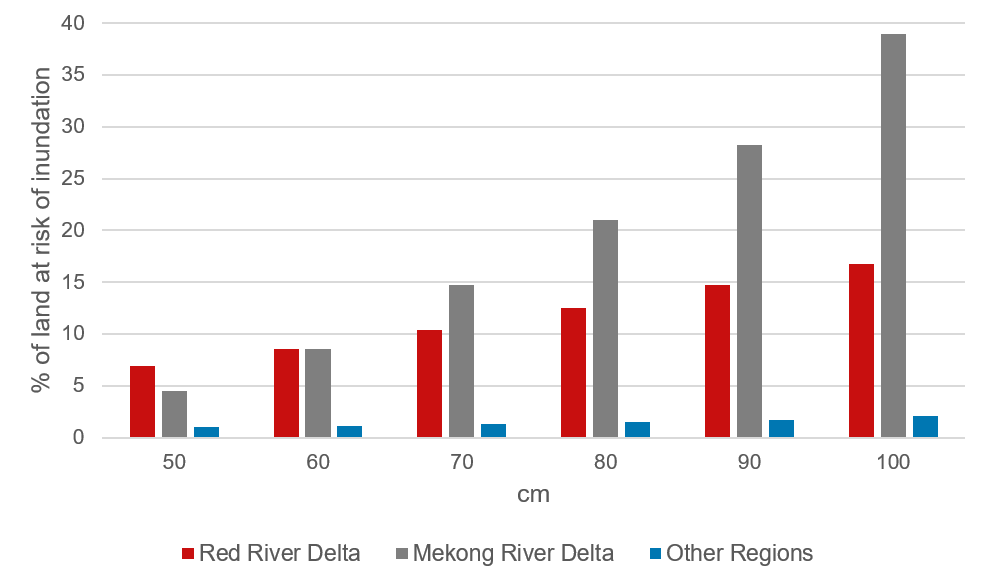
\includegraphics[width=8cm,height=5.5cm]{pictures/Sea_Level_Rise_Vietnam}
	\end{figure}
	{\footnotesize Source: \cite{thuc2016climate}}
\end{frame}

\begin{frame}<presentation>
	\frametitle{{\thesection.\thesubsection.\thesubsubsection} Cost-Benefit of Building a Dike in the Mekong River Delta (2)}
	\begin{itemize}
		\item Facts and assumptions 
		\begin{itemize}
			\item Coast line of Mekong River Delta is 600 km
			\item Dike needs to be of the same height along the entire coastline
			\item Estimated costs: 40,000 EUR for one meter height and one meter length 
			\item Height increases with sea level each year
			\item Damages associated with sea level rise in Mekong Delta River are zero, if and only if the height of the dike exceeds the sea level rise
		\end{itemize}	
		\item Benefit is defined as: difference between a scenario with dike (Adaptation) and without dike (Sea Level) relative to the Baseline scenario
	\end{itemize}
\end{frame}

\begin{frame}<presentation>
	\frametitle{{\thesection.\thesubsection.\thesubsubsection} Cost-Benefit of Building a Dike in the Mekong River Delta (3)}
	\begin{figure}
	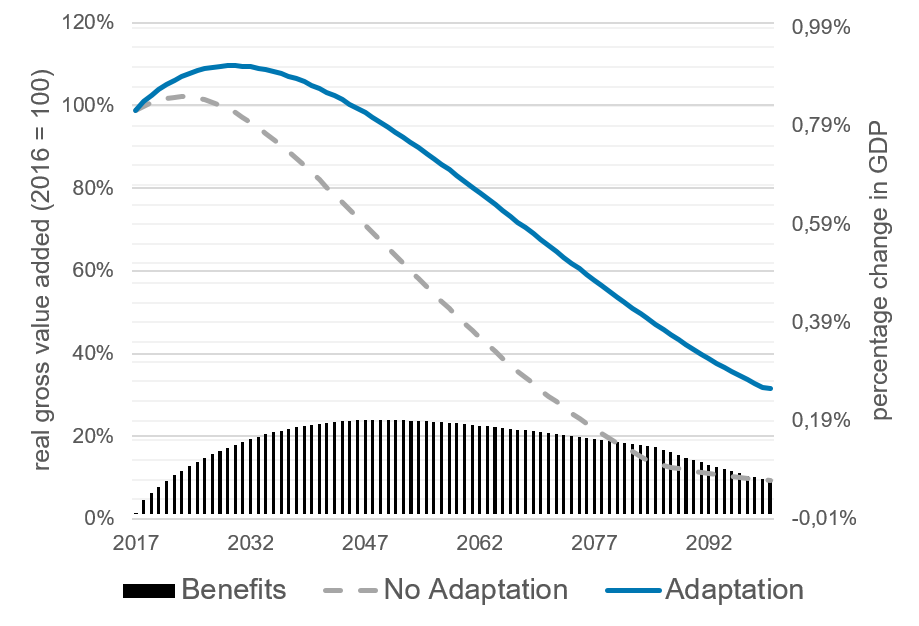
\includegraphics[width=8cm,height=5.25cm]{pictures/Cost_Benefit_Analysis_Dike}
	\end{figure}
	{\footnotesize Source: own exhibition.} \\
	{\footnotesize Note: Lines depict simulation of agricultural production and bars indicate the difference between Adaptation and No-Adaptation scenario for total GDP.}
	
\end{frame}



%%%%%%%%%%%%%%%%%%%%%%%%%%%%%%%%%%%%%%%%%%%%%%%%%%%%%%%%
\section{Model building steps}

\subsection{Definition of Scenarios}
\begin{frame}<presentation>
	\frametitle{{\thesection.\thesubsection} Definition of Climate Change Scenarios (1)}
	\begin{itemize}
		\item Determine climate change scenarios
		\item We use results from \cite{thuc2016climate} to define regional specific climate change variables
		\item Scenarios are based on the IPCC scenarios RCP 4.5 and 8.5.
		\item It is possible to define regional specific paths for:
			\begin{itemize}
				\item annual average temperature 
				\item annual average precipitation
				\item sea level rise
			\end{itemize}

	\end{itemize}
\end{frame}
\begin{frame}<presentation>
	\frametitle{{\thesection.\thesubsection} Definition of Climate Change Scenarios (2)}
	\begin{itemize}
		\item The following region specific scenarios for the climate variable temperature can be obtained using the results from Thuc et al. 2016:
		\begin{center}
			\begin{overlayarea}{8cm}{5.5cm}
				\only<1>{\includegraphics[width=7.5cm,height=5cm]{pictures/temperature/region1}\\
					\centering \footnotesize{\textit{Region 1}: Mekong River Delta}}
				\only<2>{\includegraphics[width=7.5cm,height=5cm]{pictures/temperature/region2}\\
					\centering \footnotesize{\textit{Region 2}: Red River Delta}}
				\only<3>{\includegraphics[width=7.5cm,height=5cm]{pictures/temperature/region3}\\
					\centering \footnotesize{\textit{Region 3}: North Central and Central Coast, Southeast, \linebreak Central Highlands, Northern Midlands and Mountains}}
			\end{overlayarea}
		\end{center}
	\end{itemize}
\end{frame}
\subsubsection{Wether Extremes}
\begin{frame}<presentation>
	\frametitle{{\thesection.\thesubsection.\thesubsubsection} Weather Extremes}
	\begin{itemize}
		\item \cite{thuc2016climate} do not explicitly report results for the frequency of weather extremes
		\item Define the relationship between annual averages and the frequency of weather extremes, e.g. 
			\begin{itemize}
				\item cyclones
				\item droughts
			\end{itemize}
		\item Previous studies report changes in the frequency of weather extremes for different climate change scenarios (see e.g. \cite{arndt2015economic})
	\end{itemize}
\end{frame}

\subsubsection{Baseline Scenario}
\begin{frame}<presentation>
	\frametitle{{\thesection.\thesubsection.\thesubsubsection} Baseline Scenario (1)}
	\begin{itemize}
		\item Determine a hypothetical reference path
		\item For this path no further change in climate variables
		\item Define the evolution of sectoral TFP
		\item Disentangle the impact of different impact chains on the economy
	\end{itemize}
\end{frame}


\begin{frame}<presentation>
	\frametitle{{\thesection.\thesubsection.\thesubsubsection} Baseline Scenario (2)}
	\begin{itemize}
		\item	Model parameters are set to match characteristics of Vietnamese economy in 2016
		\item	Catch-up process and transition to developed economy (Japan selected as plausible benchmark)
		\begin{itemize}
			\item	Geometric average annual growth rate set to 4\% 
			\item	Determine sectoral TFP shocks to match an assumed new long-run composition of gross value added by economic activity (agriculture 1\%, industry 35\%, services 65\%)
			\item	Long-run dynamics of labour productivity to ensure employment shares converge to values observed for developed economies
			\item	Exogenous evolution of sectoral labour and total factor productivity is completed after 120 periods
		\end{itemize}
		\item	No consideration of climate (change) effects on economic development
	\end{itemize}
\end{frame}

\subsection{Identification of Climate Hazards}

\begin{frame}<presentation>
	\frametitle{{\thesection.\thesubsection} Climate Hazards (1)}
	\begin{itemize}
		\item There are several Climate Hazards, potentially affecting Vietnam in the future
		\item Vietnam is expected to suffer from a \textit{rise in the sea level}:
		\begin{figure}
			\subfigure{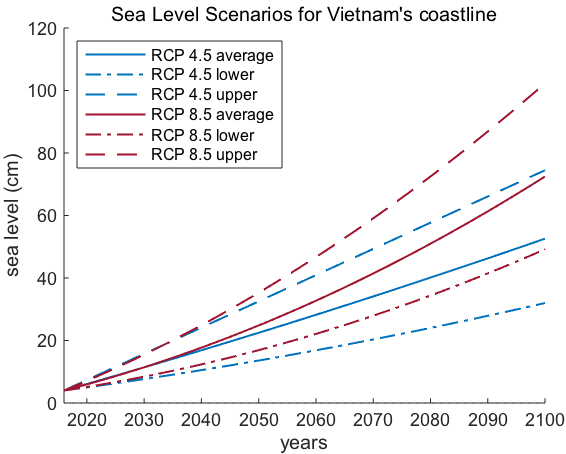
\includegraphics[width=6cm]{pictures/climate/graph_SL}}
		\end{figure}
		\hspace{2cm} \footnotesize{\textit{Source}: Own computation based on results from Thuc et al. 2016.}
	\end{itemize}
\end{frame}
\begin{frame}<presentation>
	\frametitle{{\thesection.\thesubsection} Climate Hazards (2)}
	\begin{itemize}
		\item The sea level rise will come along with a higher \textit{inundation risk} in coastal regions
		\item Example: According to Thuc et al. 2016, a sea level rise of 50mm (100mm) is expected to lead to an inundation (\% area) of
		\begin{itemize}
			\item 6.93\% (16.8\%) in the Red River Delta
			\item 4.48\% (38.9\%) in the Mekong Delta
		\end{itemize}
	\item Increases in the \textit{average temperature} are expected to cause:
		\begin{itemize}
			\item Decline of crop yield
			\item Reduction of total factor productivity
		\end{itemize}
	\item Other potential hazards: Increased frequency of \textit{cyclones}, \textit{storm surges}, etc.
	\end{itemize}
\end{frame}

\subsection{Calibration of Model Parameters}
\subsubsection{Calibration}
\begin{frame}<presentation>
	\frametitle{{\thesection.\thesubsection.\thesubsubsection} Calibration}
	\begin{itemize}
		\item	It is necessary to define structural parameters of the model to reflect the Vietnamese economy
		\item Based on identified damages and potential losses in previous studies one can calibrate functional forms of the damage functions
		\item Climate change will affect economic sectors to a different extent:
		\begin{itemize} 
			\item Previous studies show a high potential impact of agriculture, electricity markets and transportation
		\end{itemize}
	\end{itemize}
\end{frame}


\subsubsection{Scenario Analysis}
\begin{frame}<presentation>
	\frametitle{{\thesection.\thesubsection.\thesubsubsection} Scenario Analysis}
\begin{itemize}
	\item In order to gauge the impact of climate change on economic outcomes, deterministic simulations are conducted
	\item Different climate change scenarios need to be defined first, e.g. long-term projections for temperature or the sea level
	\item The model is simulated from its initial condition along the assumed climate change path
	\item Simulation results then show the adjustment processes to climate change in the economy
	\item Further, it is possible to specify adaptation measures reducing the impact of climate change on the damage function %Adaptation measures such as building damns will increase government expenditures to tackle climate change.
	\end{itemize}
\end{frame}


%%%%%%%%%%%%%%%%%%%%%%%%%%%%%%%%%%%%%%%%%%%%%%%%%%%%%%%%
\section{Introduction to Dynare}

\subsection{What is Dynare?}
\begin{frame}<presentation>
\frametitle{{\thesection.\thesubsection} What is Dynare?}
  \begin{itemize}
		\item Dynare is an open-source program for dynamic general equilibrium modeling:
		\begin{itemize}
			\item mainly a collection of different functions written for MATLAB
			\item pre-processor translates Dynare files (.mod files) into MATLAB code
		\end{itemize}
	\end{itemize}
\end{frame}

\subsection{Implementing a Model in Dynare}
\subsubsection{Neoclassical Growth Model}
\begin{frame}<presentation>
\frametitle{{\thesection.\thesubsection.\thesubsubsection} Implementing a Model in Dynare}
\framesubtitle{Neoclassical Growth Model (1)}
	 \begin{itemize}
	 	\item Households maximize lifetime utility subject to their budget constraint 
	 	\begin{gather*}
	 	\underset{\left\{ c_t, \thinspace k_{t+1}\right\} _{t=1}^{\infty}}{\max} = \sum_{t=1}^{\infty} \beta^{\thinspace t-1} \thinspace \frac{c_t^{1-\sigma}}{1-\sigma}\\
	 	\text{s.t.} \quad c_t + k_{t+1} = A_t \thinspace k_t^{\alpha} + (1-\delta) \thinspace k_t
	 	\end{gather*}
	 	\item It follows from the first order condition of the above problem with respect to consumption that the Lagrange multiplier is defined as  $$\lambda_t=\beta^{\thinspace t-1}\thinspace\sigma_t^{-\sigma},$$ representing the marginal utility of consumption
	\end{itemize}
\end{frame}
\begin{frame}<presentation>
\frametitle{{\thesection.\thesubsection.\thesubsubsection} Implementing a Model in Dynare}
\framesubtitle{Neoclassical Growth Model (2)}
	\begin{itemize}
		\item The resulting first order conditions are:
		\begin{gather*}
		c_t^{-\sigma} = \beta \thinspace c_{t+1}^{-\sigma} (\alpha \thinspace A_{t+1} \thinspace k_{t+1}^{\alpha -1} + 1 - \delta)\\[5pt]
		c_t + k_{t+1} = A_t \thinspace k_t^\alpha + (1-\delta) \thinspace k_t
		\end{gather*}
		\item By the definition $c_t=c_{t+1}=\bar{c}$ and $k_t=k_{t+1}=\bar{k}$ has to hold in the \newline steady state
		\item Therefore, the first order conditions in the steady state case become:
		\begin{gather*}
		\bar{c}^{-\sigma} = \beta \thinspace \bar{c}^{-\sigma} (\alpha \thinspace \bar{A} \thinspace \bar{k}^{\alpha -1} + 1 - \delta)\\[5pt]
		\bar{c} + \bar{k} = \bar{A} \thinspace \bar{k}^\alpha + (1-\delta) \thinspace \bar{k}
		\end{gather*}
	\end{itemize}
\end{frame}
\begin{frame}<presentation>
\frametitle{{\thesection.\thesubsection.\thesubsubsection} Implementing a Model in Dynare}
\framesubtitle{Neoclassical Growth Model (3)}
	\begin{itemize}
		\item The steady state can be obtained analytically by solving the first equation for $\bar{k}$ and the second equation for $\bar{c}$:
		\begin{gather*}
		\bar{k} = \bigg(\frac{1-\beta (1-\delta)}{\beta\thinspace\alpha\bar{A}}\bigg)^\frac{1}{\alpha -1}\\[5pt]
		\bar{c} = \bar{A} \thinspace \bar{k}^\alpha - \delta \thinspace \bar{k}		
		\end{gather*}
		\item The neoclassical growth model considered in these slides, as well as the \linebreak DGE-CRED model are \textit{deterministic models}
		\begin{itemize}
			\item No stochastic elements requiring expectancy terms or probability distributions
			\item The remainder of this introduction to Dynare focuses on this class of models
		\end{itemize}  
	\end{itemize}
\end{frame}
\subsubsection{Model File}
\begin{frame}<presentation>[fragile]
	\frametitle{{\thesection.\thesubsection.\thesubsubsection} Model File}
	\begin{itemize}
		\item A model file or mod-file (filename.mod) contains commands and blocks 
		\begin{itemize}
			\item Each command and each element of a block is terminated by a semicolon (;)
			\item Blocks are terminated by \texttt{end;} 
		\end{itemize}
		\item The model file complementary to these slides is \textit{Introduction\_Dynare.mod}
		\item Code lines within the mode file can be deactivated using \%, // or /* ... */
		\item In order to run a model file:
		\begin{itemize}
			\item The Dynare path has to be added to the search path of MATLAB
				\begin{verbatim}
				   addpath('C:\dynare\4.6.1\matlab')
				\end{verbatim}
			\item Dynare executed to run the model in MATLAB
				\begin{verbatim}
				   dynare filename
				\end{verbatim}
		\end{itemize} 
	\end{itemize}
\end{frame}

\subsubsection{Variables and Parameters}
\begin{frame}<presentation>[fragile]
	\frametitle{{\thesection.\thesubsection.\thesubsubsection} Variables and Parameters (1)}
	\begin{itemize}
		\item At the beginning of each model file, the endogenous (\texttt{var}) and exogenous (\texttt{varexo}) variables as well as parameters (\texttt{parameters}) have to be defined:
			\begin{verbatim}
			   var = c k;		
			   varexo = A;		
			   parameters alpha_p beta_p gamma_p delta_p;	
			\end{verbatim}	
		\item Then, the parameter values have to be assigned:
			\begin{verbatim}				
			   alpha_p = 0.5;
			   beta_p = 0.95;
			   gamma_p = 0.5;
			   delta_p = 0.02;
			\end{verbatim}
	\end{itemize}
\end{frame}
\begin{frame}<presentation>[fragile]
	\frametitle{{\thesection.\thesubsection.\thesubsubsection} Variables and Parameters (2)}
	\begin{itemize}
		\item Optionally, a LaTeX name and long name can be assigned to a variable using the convention:\\ 
		\begin{verbatim}
		variable_name $tex_name$ (long_name = 'quoted_string') \end{verbatim}
		\begin{itemize}
			\item Example:
		\begin{verbatim}
		  var 
		  k $k$ (long_name = 'capital'),
		  c $c$ (long_name = 'consumption');
		  
		  varexo 
		  A $A$ (long_name = 'technology');
		\end{verbatim}
		\end{itemize}
	\end{itemize}
\end{frame}
\begin{frame}<presentation>[fragile]
	\frametitle{{\thesection.\thesubsection.\thesubsubsection} Variables and Parameters (3)}
	\begin{itemize}
		\item There are some restrictions to be kept in mind, when choosing variable and parameter names in Dynare:
			\begin{itemize} 
				\item Avoid names of built-in functions and commands
				\item Minimize interface with Matlab or Octave functions
				\item Example: Do not use correctly-spelled greek letters like \texttt{beta}, instead \linebreak e.g. \texttt{betta}
			\end{itemize}
		\item Note that by convention in Dynare, the time indice of a variable refers to the period when its value is determined. The typical example is for capital stock:
			\begin{itemize}
				\item Since the capital stock entering the production function in the current period is determined in the previous period, the capital stock becomes \texttt{k(-1)}, and the law of motion of capital must be written as: \texttt{k = i + (1-delta)*k(-1)} 
				\item This convention can be modified using the \texttt{predetermined\_variables} setting
			\end{itemize}
	\end{itemize}
\end{frame}
\subsubsection{The \texttt{model} block}
\begin{frame}<presentation>[fragile]
	\frametitle{{\thesection.\thesubsection.\thesubsubsection} The \texttt{model} block}
	\begin{itemize}
		\item A model is declared inside a \texttt{model} block 
		\item In general, there must be as many equations as there are endogenous variables in the model 
		\item A great advantage of using Dynare is that the equations can be written almost as on paper
		\begin{verbatim}
		   model;
		   c + k = A*k(-1)^alpha_p + (1-delta_p)*k(-1);
		   c^(-gamma_p) = beta_p*c(+1)^(-gamma_p)
		           *(alpha_p*A(+1)*k^(alpha_p-1) + 1 - delta_p);
		   end;
		\end{verbatim}
	\end{itemize}
\end{frame}
\subsection{Steady State in Dynare}
\begin{frame}<presentation>
	\frametitle{{\thesection.\thesubsection} Steady State (1)}
	\begin{itemize}
		\item By definition a steady state of a model satisfies: $$y_t=y_{t+1}=\bar{y} \enspace \text{and} \enspace u_t=u_{t+1}=\bar{u},$$
		where $y$ is the vector of endogenous variables and $u$ the vector of exogenous shocks
		\begin{itemize}
			\item In the context of the neoclassical growth model: $y_t=(c_t \quad k_t)'$ and $u_t=A_t$
		\end{itemize}
		\item Note that a steady state is conditional to:
		\begin{itemize}
			\item The steady state values of exogenous variables $\bar{u}$
			\item The values of parameters (implicit in the above definition)
		\end{itemize}
		\item Even for a given set of exogenous and parameter values, some (nonlinear) models have several steady states
	\end{itemize}
\end{frame}
\begin{frame}<presentation>
	\frametitle{{\thesection.\thesubsection} Steady State (2)}
	\begin{itemize}
		\item The steady state is an important concept in the framework of the DGE-CRED model:
		\begin{itemize}
			\item In this model it is assumed that the economy is in steady state at the beginning of the initial period and then transits towards a new steady state, reached in the terminal period
			\item While the trajectories of the exogenous variables are given, those of the endogenous variables are determined within the model
		\end{itemize}
		\item There are three approaches to calculate the steady state in Dynare
		\item The steady state values are stored in the MATLAB matrix \texttt{oo\_.steady\_state}
	\end{itemize}
\end{frame}
\subsubsection{Approach 1}
\begin{frame}<presentation>[fragile]
	\frametitle{{\thesection.\thesubsection.\thesubsubsection} Steady State: Approach 1}
	\begin{itemize}
		\item Idea: Provide an initial guess for the steady state in the \texttt{initval} block and then conduct the steady state calculation using \texttt{steady}
		\item Example, considering the neoclassical growth model:
		\begin{verbatim}
		   initval;
		   c = 2;
		   k = 30;
		   A = 1;
		   end;
		   steady;
		\end{verbatim}
	\end{itemize}
\end{frame}
\subsubsection{Approach 2}
\begin{frame}<presentation>[fragile]
	\frametitle{{\thesection.\thesubsection.\thesubsubsection} Steady State: Approach 2 (1)}
	\begin{itemize}
		\item Idea: Use a \texttt{steady\_state\_model} block, in which the steady state values are calculated
		\item Example, considering the neoclassical growth model:
		\begin{verbatim}
		   initval;
		   A = 1;
		   end;		
		   steady_state_model;
		   k = ((1 - beta_p*(1 - delta_p))/
		          (beta_p*alpha_p*A))^(1/(alpha_p - 1));
		   c = A*k^alpha_p - delta_p*k;
		   end;
		\end{verbatim}
	\end{itemize}
\end{frame}
\begin{frame}<presentation>[fragile]
	\frametitle{{\thesection.\thesubsection.\thesubsubsection} Steady State: Approach 2 (2)}
	\begin{itemize}
		\item Note that the steady state values of the exogenous variables have to be assigned in an \texttt{initval} block
		\item In cases where the steady state can be solved analytically, using a \texttt{steady\_state\_model} block is a suitable approach
	\end{itemize}
\end{frame}
\subsubsection{Approach 3}
\begin{frame}<presentation>[fragile]
	\frametitle{{\thesection.\thesubsection.\thesubsubsection} Steady State: Approach 3 (1)}
	\begin{itemize}
		\item Idea: Use an explicit steady state file, which is an external MATLAB-file that must conform with a certain structure and naming convention:\\ \texttt{NAMEofMODfile\_steadystate.m}
		\item In this steady state file, you must provide the exact steady state values as in the case of the \texttt{steady\_state\_model} block
		\item Note: A steady state file is used in the DGE--CRED model
	\end{itemize}
\end{frame}
\begin{frame}<presentation>[fragile]
	\frametitle{{\thesection.\thesubsection.\thesubsubsection} Steady State: Approach 3 (2)}
	\begin{itemize}
		\item Advantage: 
		\begin{itemize}
			\item Flexibility, can call build-in MATLAB functions
			\item Allows for changing parameters to take parameter dependencies into account without resorting to model-local variables
		\end{itemize}
		\item Drawback: 
		\begin{itemize}
			\item Additional flexibility offered by a steady state file increases the scope for errors
		\end{itemize} 
	\end{itemize}
\end{frame}
\subsection{Deterministic Simulations in Dynare}
\subsubsection{Deterministic Simulation}
\begin{frame}<presentation>[fragile]
	\frametitle{{\thesection.\thesubsection.\thesubsubsection} Deterministic Simulation (1)}
	\begin{itemize}
		\item The deterministic simulation builds up on the concept of \textit{perfect foresight}, in which agents have full knowledge and perfectly anticipate all future shocks
		\item More precisely, we assume that:
		\begin{itemize}
			\item Agents learn the value of all future shocks
			\item Since there is shared knowledge of the model and of future shocks, agents can compute their optimal plans for all future periods
			\item optimal plans are not adjusted in periods 2 and later\\ $\Rightarrow$ the model behaves as if it were deterministic
		\end{itemize}
		\item Cost of this approach: The effect of future uncertainty is not taken into account
		\item Advantage: Numerical solutions can be computed exactly (up to rounding errors) and nonlinearities are fully taken into account
	\end{itemize}
\end{frame}
\begin{frame}<presentation>
	\frametitle{{\thesection.\thesubsection.\thesubsubsection} Deterministic Simulation (2)}
	\begin{itemize}
		\item The general problem in the deterministic, perfect foresight, case can be expressed as: $$f(y_{t+1},y_t,y_{t-1},u_t)=0,$$ where $y$ is the vector of endogenous variables and $u$ the vector of exogenous shocks
		\item Identification rule: There must be as many equations in $f(...)$ as there are endogeneous variables in $y$
		\item The general perfect foresight problem for the neoclassical growth model is:
		\begin{gather*}
		f(y_{t+1},y_t,y_{t-1},u_t) = \begin{pmatrix} 	c_t^{-\sigma} - \beta  \thinspace c_{t+1}^{-\sigma} (\alpha \thinspace A_{t+1}  \thinspace k_{t+1}^{\alpha -1} + 1 - \delta)\\ c_t + k_{t+1} - A_t  \thinspace k_t^\alpha - (1-\delta)  \thinspace k_t \end{pmatrix} = \begin{pmatrix}
		0 \\0
		\end{pmatrix},
		\end{gather*}
		where $y_t = (c_t \enspace k_{t+1})'$ and $u_t = A_t$
	\end{itemize}
\end{frame}
\begin{frame}<presentation>
	\frametitle{{\thesection.\thesubsection.\thesubsubsection} Deterministic Simulation (3)}
	\begin{itemize}
		\item The aim of a deterministic simulation is to examine the trajectories of the model variables over the time period $t = 1,...,T$
		\item Consequently, the stacked system for a perfect foresight simulation over $T$ periods becomes a two-boundary value problem: 
		$$\left\{ \begin{matrix} f(y_2,y_1,\mathbin{\textcolor{red}{y_0}},\mathbin{\textcolor{blue}{u_1}})=0 \\ 
		f(y_3,y_2,y_1,\mathbin{\textcolor{blue}{u_2}})=0 \\ 
		\vdots \\ 
		f(\mathbin{\textcolor{red}{y_{T+1}}},y_T,y_{T-1},\mathbin{\textcolor{blue}{u_T}})=0 
		\end{matrix},  \right.$$ 
		where $y_0$ and $y_{T+1}$ as well as $u_1,...,u_T$ are given
		\item Dynare uses a Newton-type methode to solve this stacked system
	\end{itemize}
\end{frame}
\begin{frame}<presentation>
	\frametitle{{\thesection.\thesubsection.\thesubsubsection} Deterministic Simulation (4)}
	\begin{itemize}
		\item The Newton method numerically solves the two-boundary value problem and hence computes trajectories for given shocks over a \textit{finite} number of periods
		\item If one is rather interested in solving an \textit{infinite}-horizon problem:
		\begin{itemize}
			\item The easiest way is to approximate the solution by a finite-horizon problem \linebreak (large $T$)
			\item Drawback: The solution is specific to a given sequence of shocks, and not generic
		\end{itemize} 
	\end{itemize}
\end{frame}
\begin{frame}<presentation>
	\frametitle{{\thesection.\thesubsection.\thesubsubsection} Deterministic Simulation (5)}
	\begin{itemize}  
		\item In case there is more than one lead or lag, Dynare automatically transforms the model in the form with one lead and one lag using auxiliary variables 
		\item For example, if there is a variable with two leads $x_{t+2}$:
		\begin{itemize}
			\item create a new auxiliary variable $a$
			\item replace all occurrences of $x_{t+2}$ by $a_{t+1}$
			\item add a new equation: $a_t = x_{t+1}$		
		\end{itemize}
	\end{itemize}
\end{frame}
\subsubsection{Newton Method}
\begin{frame}<presentation>
	\frametitle{{\thesection.\thesubsection.\thesubsubsection} Newton Method (1)}
	\begin{itemize}
		\item The following slides aim to provide an intuition for the Newton method used by the perfect foresight solver in Dynare
		\item Start from an initial guess $Y^{(0)}$, where $Y=[y_1' \quad y_2' \enspace \ldots \enspace y_T']'$
		\item Iterate: Updated solutions $Y^{(k+1)}$ are obtained by solving a linear system 
		$$F(Y^{k}) + \bigg[\frac{\partial F}{\partial Y}\bigg] (Y^{(k+1)} - Y^{(k)}) = 0$$
	\end{itemize}
\end{frame}
\begin{frame}<presentation>
	\frametitle{{\thesection.\thesubsection.\thesubsubsection} Newton Method (2)}
	\begin{itemize}
		\item Terminal condition for the solver:
		$$\Vert Y^{(k+1)} - Y^{(k)} \Vert < \epsilon_Y$$
		or
		$$\Vert F(Y^{(k)}) \Vert < \epsilon_F$$
		\item Convergence may never happen if function is ill-behaved or initial guess $Y^{(0)}$ is too far from solution\\
		$\Rightarrow$ to avoid an infinite loop, abort after a given number of iterations
	\end{itemize}
\end{frame}
\begin{frame}<presentation>
	\frametitle{{\thesection.\thesubsection.\thesubsubsection} Newton Method (3)}
	\begin{itemize}
		\item The following options to the \texttt{perfect\_foresight\_solver} can be used to control the Newton algorithm:\\
		\begin{itemize}
			\item \texttt{maxit}: Maximum number of iterations before aborting (default: 50)
			\item \texttt{tolf}: Convergence criterion based on function value ($\epsilon_F$) (default: $10^{-5}$ 
			\item \texttt{tolx}: Convergence criterion based on change in function argument ($\epsilon_Y$) (default: $10^{-5}$)
			\item \texttt{stack\_solver\_algo}: Select between the different flavors of Newton algorithms
		\end{itemize}
	\end{itemize}
\end{frame}
\subsection{Perfect Foresight Setup in Dynare}
%\paragraph{Getting stated with Perfect Foresight}
\subsubsection{Introduction}
\begin{frame}<presentation>[fragile]
	\frametitle{{\thesection.\thesubsection.\thesubsubsection} Introduction}
	\begin{itemize}
		\item In order to perform the deterministic simulation, one has to specify:
		\begin{itemize}
			\item The constraints of the stacked system $y_0$, $y_{T+1}$ and $u_1, \ldots , u_T$
			\item Provide an initial guess $y_1, \ldots , y_T$ for the Newton algorithm 
		\end{itemize} 
		\item The path for the endogenous and exogenous variables are stored in two MATLAB/Octave matrices:
		\begin{itemize}
			\item \texttt{oo\_.endo\_simul = ($y_0$  $y_1$ \ldots \enspace  $y_T$  $y_{T+1}$)}
			\item \texttt{oo\_.exo\_simul' = ($y_0$  $y_1$ \ldots \enspace  $y_T$  $y_{T+1}$)}
		\end{itemize}
		\item The \texttt{perfect\_foresight\_setup} initializes those matrices, given the \texttt{shocks}, \texttt{initval}, \texttt{endval} and \texttt{histval} blocks
		\item Then, the \texttt{perfect\_foresight\_solver} replaces $y_1,\ldots,y_T$ by the solution 
	\end{itemize}
\end{frame}
\subsubsection{Transition from an Initial to a Terminal Steady State}
\begin{frame}<presentation>[fragile]
	\frametitle{{\thesection.\thesubsection.\thesubsubsection} Transition from an Initial to a Terminal Steady State (1)}
	\begin{itemize}
		\item The following slides examine a specific type of deterministic simulation, which is needed in the DGE-CRED framework 
		\item The DGE-CRED Model allows its user to investigate:
		\begin{itemize}
			\item The trajectories of the endogenous variables
			\item Given the parameter values and pathways of the exogenous variables
		\end{itemize} 
		\item It is assumed that the economy is:
		\begin{itemize}
			\item In an inital steady state at the beginning of the model period $(t=0)$
			\item Transits towards a new steady state in the terminal period $(t=T+1)$
		\end{itemize}
	\end{itemize}
\end{frame}
\begin{frame}<presentation>[fragile]
	\frametitle{{\thesection.\thesubsection.\thesubsubsection} Transition from an Initial to a Terminal Steady State (2)}
	\begin{itemize}
		\item In order to implement this specific type of deterministic simulation, the following can be conducted in Dynare:
		\begin{itemize}
			\item Use a steady state file. This enables a steady state computation for varying values of the exogenous variables and allows using numeric solvers.
			\item Declare the initial values of the exogenous variables in an \texttt{initval} block followed by \texttt{steady}.
			\item Declare the terminal values of the exogenous variables in an \texttt{endval} block followed by \texttt{steady}.
			\item Note: This is basically the same idea as presented in ``approach 3'' of the section covering the steady state calculation.
		\end{itemize}
	\end{itemize}
\end{frame}
\begin{frame}<presentation>[fragile]
	\frametitle{{\thesection.\thesubsection.\thesubsubsection} Transition from an Initial to a Terminal Steady State (3)}
	\begin{itemize}
		\item The initial steady state values are determined based on the values of the exogenous variables assigned in the \texttt{initval} block 
		\begin{itemize}
			\item These values are then stored as initial values in \texttt{oo\_.endo\_simul} and \texttt{oo\_.exo\_simul}
		\end{itemize}
		\item The terminal steady state values are determined based on the values of the exogenous variables assigned in the \texttt{endval} block 
		\begin{itemize}
			\item These values are then stored as terminal values as well as initial guess for the numerial solver in \texttt{oo\_.endo\_simul} and \texttt{oo\_.exo\_simul}
		\end{itemize}
	\end{itemize}
\end{frame}
\begin{frame}<presentation>[fragile]
	\frametitle{{\thesection.\thesubsection.\thesubsubsection} Transition from an Initial to a Terminal Steady State (4)}
	\begin{itemize}
		\item Example: The economy starts from the initial steady state, where $A_0=1$. In the terminal steady state, the total factory productivity is 10\% higher.
		\begin{verbatim}
		   initval;
		   A = 1;
		   end; 
		   steady;
		
		   endval;
		   A = 1.1;
		   end;
		   steady;
		\end{verbatim}
	\end{itemize}
\end{frame}
\begin{frame}<presentation>[fragile]
	\frametitle{{\thesection.\thesubsection.\thesubsubsection} Transition from an Initial to a Terminal Steady State (5)}
	\begin{itemize}
		\item The following trajectories are obtained:
		\begin{figure}
			\centering
			\subfigure{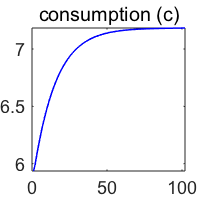
\includegraphics[width=3.5cm]{pictures/transition/consumption_transition}}\qquad
			\subfigure{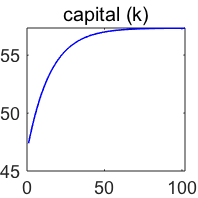
\includegraphics[width=3.5cm]{pictures/transition/capital_transition}}\qquad
			\subfigure{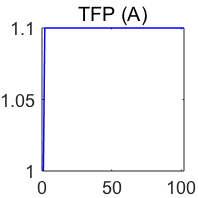
\includegraphics[width=3.5cm]{pictures/transition/TFP_transition}}
		\end{figure}
	\end{itemize}
\end{frame}
\subsubsection{The \texttt{initval} Block}
\begin{frame}<presentation>
	\frametitle{{\thesection.\thesubsection.\thesubsubsection} The \texttt{initval} Block (1)}
	\begin{itemize}
		\item While the previous slides examined the usage of the \texttt{initval} and \texttt{endval} block in combination with \texttt{steady}, these blocks have more functionalities than encountered so far
		\item In presence of the \texttt{initval} and absence of other blocks:
		\begin{itemize}
			\item \texttt{oo\_.endo\_simul} and \texttt{oo\_.exo\_simul} variables storing the endogenous and exogenous variables will be filled with the values provided by this block
			\item It will therefore provide the initial and terminal conditions for all the endogenous and exogenous variables
			\item For the intermediate simulation periods it provides the starting values for the solver 
		\end{itemize} 
		\item It is important to be aware that if some variables, endogenous or exogenous, are not mentioned in the \texttt{initval} block, a zero value is assumed
	\end{itemize}
\end{frame}
\begin{frame}<presentation>[fragile]
	\frametitle{{\thesection.\thesubsection.\thesubsubsection} The \texttt{initval} Block (2)}
	\begin{itemize}
		\item Example: Let us assume that we want to set $c_0=c_{T+1}=4$ and $k_0=k_{T+1}=20$ in the neoclassical growth model. Furthermore, we assume that TFP is constant at $A_t=1$.
			\begin{verbatim}
				   initval;
				   c = 4;
				   k = 20;
				   A = 1;
				   end;
			\end{verbatim}
		\item Note that the purpose of this example is to illustrate the usage of the \texttt{initval} block, rather than adressing a meaningful question.
	\end{itemize}
\end{frame}
\begin{frame}<presentation>[fragile]
	\frametitle{{\thesection.\thesubsection.\thesubsubsection} The \texttt{initval} Block (3)}
	\begin{itemize}
		\item In order to run the deterministic simulation for $T=100$ periods, enter:
		\begin{verbatim}
		perfect_foresight_setup(periods=100);
		perfect_foresight_solver;
		\end{verbatim}
	\end{itemize}
\end{frame}
\begin{frame}<presentation>[fragile]
	\frametitle{{\thesection.\thesubsection.\thesubsubsection} The \texttt{initval} Block (4)}
	\framesubtitle{The \texttt{initval} Block (4)}
	\begin{itemize}
		\item The following trajectories are obtained:
		\begin{figure}
			\centering
			\subfigure{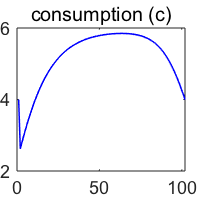
\includegraphics[width=3.5cm]{pictures/consumption01}}\qquad
			\subfigure{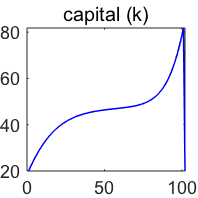
\includegraphics[width=3.5cm]{pictures/capital01}}\qquad
			\subfigure{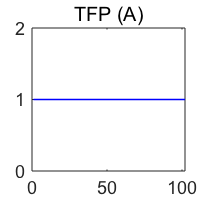
\includegraphics[width=3.5cm]{pictures/TFP01}}
		\end{figure}
		\item Comments:
			\begin{itemize}
				\item As consumption is a forward looking variable in this model, its initialization $c_0$ does not affect the trajectory. However, its terminal value does.
				\item The opposite holds for capital. 
			\end{itemize}
	\end{itemize}
\end{frame}
%\paragraph{The \texttt{endval} block}
\subsubsection{The \texttt{endval} Block}
\begin{frame}<presentation>[fragile]
	\frametitle{{\thesection.\thesubsection.\thesubsubsection} The \texttt{endval} Block (1)}
	\begin{itemize}
		\item In the absence of an \texttt{initval} block, the \texttt{endval} block fills both\linebreak \texttt{oo\_.endo\_simul} and \texttt{oo\_.exo\_simul}
		\begin{itemize}
			\item In this case it, therefore, has the same effect as if only an \texttt{initval} block was present
		\end{itemize}
		\item However, if an \texttt{initval} and  \texttt{endval} block are both present:
		\begin{itemize}
			\item The former assigns the initial conditions in $t=0$
			\item While the latter provides the terminal conditions in $t=T+1$ as well as the initial guess for the perfect foresight solver
		\end{itemize} 
		\item Example: Let us assume that we want to set $c_0=4$, $c_{T+1}=6$, $k_0=20$, $k_{T+1}=30$ and $A_t=1$
		\item As before, the purpose of this example is to illustrate the usage of the \texttt{endval} block, rather than adressing a meaningful question
	\end{itemize}
\end{frame}
\begin{frame}<presentation>[fragile]
	\frametitle{{\thesection.\thesubsection.\thesubsubsection} The \texttt{endval} Block (2)}
	\begin{itemize}
		\item Leading the following code:
			\begin{verbatim}
			   initval;
			   c = 4;
			   k = 20;
			   A = 1;
			   end;

			   endval;
			   c = 6;
			   k = 30;
			   A = 1;
			   end;
			\end{verbatim}
	\end{itemize}
\end{frame}
\begin{frame}<presentation>[fragile]
	\frametitle{{\thesection.\thesubsection.\thesubsubsection} The \texttt{endval} Block (3)}
		\begin{itemize}
		\item The following trajectories are obtained:
		\begin{figure}
			\centering
			\subfigure{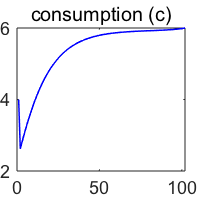
\includegraphics[width=3.5cm]{pictures/consumption02}}\qquad
			\subfigure{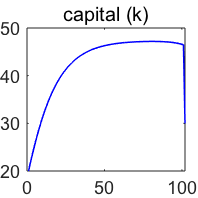
\includegraphics[width=3.5cm]{pictures/capital02}}\qquad
			\subfigure{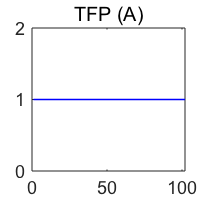
\includegraphics[width=3.5cm]{pictures/TFP02}}
		\end{figure}
		\item Comment: As in the previous example, consumption is forward looking, while capital is backward looking.
	\end{itemize}
\end{frame}
\subsubsection{The \texttt{histval} Block}
\begin{frame}<presentation>[fragile]
	\frametitle{{\thesection.\thesubsection.\thesubsubsection} The \texttt{histval} Block (1)}
	\begin{itemize}
		\item The usage of the \texttt{histval} block is particularly interesting, if there are variables with more than one lead or lag 
		\item In a deterministic simulation the \texttt{histval} block must be combined with an \texttt{initval} block 
		\item A \texttt{histval} and \texttt{endval} block cannot be combined
		\item The \texttt{histval} block assigns the initial condition, while the \texttt{initval} block provides the terminal condition and inital guess for the perfect foresight solver
	\end{itemize}
\end{frame}
\begin{frame}<presentation>[fragile]
	\frametitle{{\thesection.\thesubsection.\thesubsubsection} The \texttt{histval} Block (2)}
	\begin{itemize}
		\item The previous example can, therefore, also be implemented by:
			\begin{verbatim}
				   histval;
				   c(0) = 4;
				   k(0) = 20;
				   A(0) = 1;
				   end;
				
				   initval;
				   c = 6;
				   k = 30;
				   A = 1;
				   end;
			\end{verbatim}
	\end{itemize}
\end{frame}
\subsubsection{Shocks on Exogenous Variables}
\begin{frame}<presentation>[fragile]
	\frametitle{{\thesection.\thesubsection.\thesubsubsection} Shocks on Exogenous Variables (1)}
	\begin{itemize}
		\item For deterministic simulations, the \texttt{shocks} block specifies temporary changes in the value of exogenous variables 
		\item For permanent shocks, use an \texttt{endval} block
		\item It is possible to specify shocks which last several periods and which can vary over time  
		\begin{itemize}
			\item The \texttt{periods} keyword accepts a list of several dates or date ranges, which must be matched by as many shock values in the \texttt{values} keyword
		\end{itemize}
		\item Note that a range in the \texttt{periods} keyword can be matched by only one value in the \texttt{values} keyword  
		\begin{itemize}
			\item If values represents a scalar, the same value applies to the whole range
			\item If values represents a vector, it must have as many elements as there are periods in the range
		\end{itemize}
	\end{itemize}
\end{frame}
\begin{frame}<presentation>[fragile]
	\frametitle{{\thesection.\thesubsection.\thesubsubsection} Shocks on Exogenous Variables (2)}
	\begin{itemize}
		\item The \texttt{shock} block has the following structure:
			\begin{verbatim}
			   shocks;
			   var ... ;
			   periods ... ;
			   values ... ;
			   end;
			\end{verbatim}
		\item Examples using the \texttt{shock} block will be examined at the end of this section
	\end{itemize}
\end{frame}
\subsection{Remarks and Examples}
\subsubsection{Remarks}
\begin{frame}<presentation>[fragile]
	\frametitle{{\thesection.\thesubsection.\thesubsubsection} Remarks}
	\begin{itemize}
		\item Because of the various functions of the \texttt{initval}, \texttt{endval} and \texttt{histval} blocks, it is strongly recommended to check the constructed \texttt{oo\_.endo\_simul} and \texttt{oo\_.exo\_simul} variables after running \texttt{perfect\_foresight\_setup} and before running \texttt{perfect\_foresight\_solver} 
		\item \texttt{simul(periods = T}) executes both,  \texttt{perfect\_foresight\_setup} and \linebreak \texttt{perfect\_foresight\_solver} at the same time and can also be used
		\item The following slides cover some examples based on the neoclassical growth model 
		\begin{itemize}
			\item It is recommendable to take a look at the file \textit{Introduction\_Dynare.mod} while proceeding with these examples
		\end{itemize}
	\end{itemize}
\end{frame}
\subsubsection{Examples}
\begin{frame}<presentation>[fragile]
	\frametitle{{\thesection.\thesubsection.\thesubsubsection} Example No. 1}
	\begin{itemize}
		\item Scenario 1: Return to equilibrium starting from $k_0=0.5\bar{k}$.
			\begin{verbatim}
			   ...
			   steady;
			   
			   ik = varlist_indices('k',M_.endo_names);
			   kstar = oo_.steady_state(ik);
			   
			   histval;
			   k(0) = kstar/2;
			   end;
			   ...
			\end{verbatim}
	\end{itemize}
\end{frame}
\begin{frame}<presentation>[fragile]
	\frametitle{{\thesection.\thesubsection.\thesubsubsection} Example No. 2}
	\begin{itemize}
		\item Scenario 2: The economy starts from the steady state. There is an unexpected positive productivity shock at the beginning of period 1: $A_1 = 1.1$.
		\begin{verbatim}
		   ...
		   steady;
		
		   shocks;
		   var A;
		   periods 1;
		   values 1.1;
		   end;
		   ...
		\end{verbatim}
	\end{itemize}
\end{frame}
\begin{frame}<presentation>[fragile]
	\frametitle{{\thesection.\thesubsection.\thesubsubsection} Example No. 3}
	\begin{itemize}
		\item Scenario 3: The economy starts from the steady state. There is a sequence of shocks to $A_t$: 10\% in period 5 and an additional 5\% during the 4 following periods.
		\begin{verbatim}
	  	...
		   steady;
		
		   shocks;
		   var A;
		   periods 4, 5:8;
		   values 1.1, 1.05;
		   end;
		   ...
		\end{verbatim}
	\end{itemize}
\end{frame}
\begin{frame}<presentation>[fragile]
	\frametitle{{\thesection.\thesubsection.\thesubsubsection} Example No. 4}
	\begin{itemize}
		\item Scenario 4: The economy starts from the initial steady state. In period 6, TFP increases by 10\% permanently. 
			\begin{itemize}
				\item Same \texttt{initval} and \texttt{endval} blocks as in Scenario 4.
				\item A shock block is used to maintain TFP at its initial level during periods 1-5.
			\end{itemize}
		\begin{verbatim}
		   ...
		   shocks;
		   var A;
		   periods 1:5;
		   values 1;
		   end;
		   ...
		\end{verbatim}
	\end{itemize}
\end{frame}

\subsection{Macro Processor}
\subsubsection{Macro Language}
\begin{frame}<presentation>
	\frametitle{{\thesection.\thesubsection.\thesubsubsection} Macro-processing Language (1)}
	\begin{itemize}
		\item So far, we have encountered the \textbf{Dynare language} (used in mod-files), which is well suited for many economic models. 
		\begin{itemize}
			\item The Dynare language is a markup language for MATLAB/Octave that defines models,
			\item but itself lacks a programmatic element.
		\end{itemize}
		\item The \textbf{Dynare macro language} adds a programmatic element to Dynare.
		\begin{itemize}
			\item It allows to replicate blocks of equations through loops (\texttt{for} structure), conditionally executing some code (\texttt{if/then/else} structure), writing indexed sums or products inside equations, etc.
			\item It is used to speed model development,
			\item and useful in various situations. Examples: Multi-region models, creation of modular mod-files, variable flipping, conditional inclusion of equations, etc.
		\end{itemize}
	\end{itemize}
\end{frame}
\begin{frame}<presentation>
	\frametitle{{\thesection.\thesubsection.\thesubsubsection} Macro-processing Language (2)}
	\begin{itemize}
		\item The Dynare macro language provides a new set of \textbf{macro commands} that can be used in mod-files
		\item Technically, this macro language is totally independent of the basic Dynare language, and is processed by a seperate component of the Dynare pre-processor
		\item This macro processor transforms a mod-file with macros into a mod-file without macros (doing text expansion/inclusions) and then feeds it to the Dynare parser
		\item The key point is to understand that the macro processor only does text substitution (like the C preprocessor or the PHP language)
	\end{itemize}
\end{frame}
\begin{frame}<presentation>
	\frametitle{{\thesection.\thesubsection.\thesubsubsection} Macro-processing Language (3)}
	\begin{itemize}
		\item The flowchart below illustrates the relation between the Dynare macro language, macro processor, Dynare language and MATLAB/Octave
		\begin{figure}
			\centering
			\subfigure{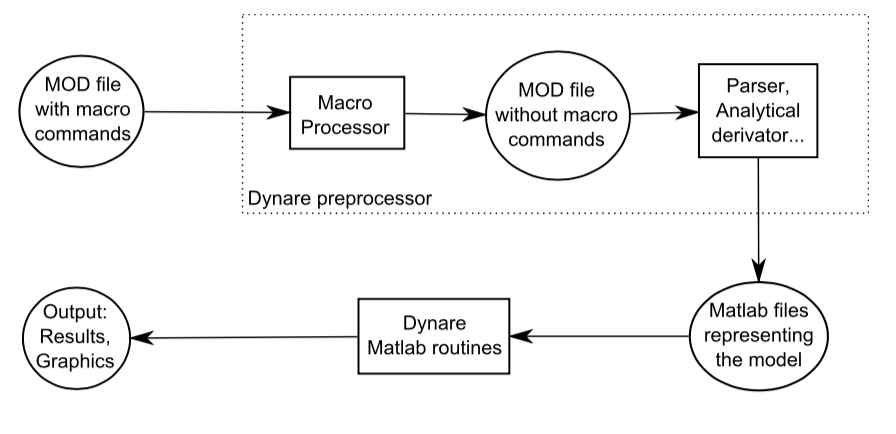
\includegraphics[width=10cm]{pictures/flowchart_macroprocessor}}
		\end{figure}
	\hspace{1.75cm} \tiny{\textit{Source}: Villemot, S. and H. Bastani: ``The Dynare Macro Processor - Dynare Summer School 2019''.}
	\end{itemize}
\end{frame}
\subsubsection{Introduction to the Syntax}
\begin{frame}<presentation>
	\frametitle{{\thesection.\thesubsection.\thesubsubsection} Introduction to the Syntax (1)}
	\begin{itemize}
		\item The macro-processor is invoked by placing \textit{macro directives} in the mod-file
		\item Directives begin with: \texttt{@\#}  
		\item The main directives are:
		\begin{itemize}
			\item \texttt{@\#include}: file inclusion
			\item \texttt{@\#define}: definition of a macro processor variable
			\item \texttt{@\#if, @\#ifdef, @\#ifndef, @\#else, @\#endif}: conditional statements
			\item \texttt{@\#for/@\#endfor}: loop statements 
		\end{itemize}
	\item Most directives fit on one line
	\item If needed however, two backslashes at the end of a line indicate that the directive is continued on the next line
	\end{itemize}
\end{frame}
\begin{frame}<presentation>
	\frametitle{{\thesection.\thesubsection.\thesubsubsection} Introduction to the Syntax (2)}
	\begin{itemize}
		\item The macro processor has its own list of variables which are different than model variables and MATLAB/Octave variables
		\item There are 4 types of macro-variables:
		\begin{itemize}
			\item integer 
			\item string 
			\item integer array 
			\item string array
		\end{itemize}
		\item Note that there is no boolean type:
		\begin{itemize}
			\item false is represented by integer zero
			\item true is any non-zero integer
		\end{itemize} 
		\item As the macro-processor cannot handle non-integer real numbers, integer division results in the quotient with the fractional part truncated (hence, $5/3=3/3=1$)
	\end{itemize}
\end{frame}
\begin{frame}<presentation>
	\frametitle{{\thesection.\thesubsection.\thesubsubsection} Introduction to the Syntax (3)}
	\begin{itemize}
		\item The following slides introduce the directives used in the DGE-CRED model
		\begin{itemize}
			\item In order to be able to use and modify the DGE-CRED, it is sufficient to master these commands
		\end{itemize} 
		\item The sources listed below encompass a comprehensive explanation of the \textit{entire} syntax of the macro language:
		\begin{itemize}
			\item Villemot, S. and H. Bastani: ``The Dynare Macro Processor - Dynare Summer School 2019''
			\item Chapter 4.24 in Dynare Reference Manual Version 4
		\end{itemize}
	\end{itemize}
\end{frame}
\begin{frame}<presentation>[fragile]
	\frametitle{{\thesection.\thesubsection.\thesubsubsection} Introduction to the Syntax (4)}
	\begin{itemize}
		\item The value of a macro-variable can be defined with the \texttt{@\#define} directive
		\begin{verbatim}
		   @#define Regions = 3
		\end{verbatim}
		\item Macro-expressions can be used in two places:
		\begin{itemize}
			\item Inside a macro directive; no special markup is required (as in the example above)
			\item In the body of the mod-file, between an at sign and curly braces (like \texttt{@{expr}}); the macro processor will substitute the expression with its value:
				\begin{verbatim}
				   parameters z;
				   z = @{Regions};
				\end{verbatim}
			In the example above the value of 3 is assigned to parameter z
		\end{itemize}
	\end{itemize}
\end{frame}
\begin{frame}<presentation>[fragile]
	\frametitle{{\thesection.\thesubsection.\thesubsubsection} Introduction to the Syntax (5)}
	\begin{itemize}
		\item The \texttt{include} directive simply inserts the text of another file in its place
		\begin{verbatim}
		   @#include "ModFiles/DGE_CRED_Model_Equations.mod"
		\end{verbatim}
		\item It is equivalent to copy/paste of the content of the included file
		\item Note that it is possible to nest includes (i.e. to include a file with an include file)
		\item Files to include are searched for in the current directory. Other directories can be added with the \texttt{@\#includepath} directive
	\end{itemize}
\end{frame}
\begin{frame}<presentation>[fragile]
	\frametitle{{\thesection.\thesubsection.\thesubsubsection} Introduction to the Syntax (6)}
	\begin{itemize}
		\item Loops can be implemented using the \texttt{@\#for...@\#endfor} directive
		\item In a model encompassing multiple regions, loops can faciliate setting up a \text{model} block:
		\begin{verbatim}
		   model;
		   @#for reg in 1:Regions
		        Y_@{reg} = A_@{reg} * (K_@{reg})^alpha 
		                            * (L_@{reg})^(1-alpha);
		   @#endfor
		   ...
		   end;
		\end{verbatim}
	\end{itemize}
\end{frame}
\begin{frame}<presentation>[fragile]
	\frametitle{{\thesection.\thesubsection.\thesubsubsection} Introduction to the Syntax (7)}
	\begin{itemize}
		\item The previous example also illustrates a great advantage of the macro language compared to the MATLAB/Ocatve syntax 
		\begin{itemize}
			\item In MATLAB it is not possible to change the index of a variable, for example $Y_r,K_r,L_r$
			\item Intuition: The Dynare macro as well as basic language rather have the character of a text than code, which is then transforemed by Dynare and MATLAB into a code
			\item It is also possible to use the MATLAB syntax directly in a mod-file. Dynare simply does not have to translate this part of the file further
		\end{itemize}
	\end{itemize}
\end{frame}
\begin{frame}<presentation>[fragile]
	\frametitle{{\thesection.\thesubsection.\thesubsubsection} Introduction to the Syntax (8)}
	\begin{itemize}
		\item The most basic conditional directive is the if-statement 
		\begin{itemize}
			\item It is executed by the directive \texttt{@\#if,...,@\#else,@\#endif}
		\end{itemize}
		\begin{verbatim}
		   @#define RCP_scenario = 4.5 // choose: 4.5 or 8.5
		   parameters Temp_2100;
		   ...
		   @#if RCP_scenario == 4.5
		   	   Temp_2100 = 2.3;
		   @#else
		   	   Temp_2100 = 3.9;
		   @#endif
		\end{verbatim}
	\end{itemize}
\end{frame}
\begin{frame}<presentation>[fragile]
	\frametitle{{\thesection.\thesubsection.\thesubsubsection} Introduction to the Syntax (9)}
	\begin{itemize}
		\item In the example on the previous slide, \texttt{Temp\_2100} is a parameter representing the temperature in 2100 
		\begin{itemize}
			\item Its value is assigned using a conditional statement
		\end{itemize}
		\item The lines between \texttt{@\#if}, \texttt{@\#else} or \texttt{@\#endif} are executed only if the condition evaluates to a non-null integer (i.e. is true) 
		\item The \texttt{@\#else} branch is optional and, if present, is only evaluated if all other conditions evaluate to 0 (i.e. do not hold)
	\end{itemize}
\end{frame}

\section{DGE--CRED Model}

\subsection{Introduction}
\begin{frame}<presentation>
\frametitle{{\thesection.\thesubsection} Introduction}
\begin{itemize}
\item Dynamic general equilibrium (DGE) model with optimizing agents.
\item Differentiates between several regions and main economic activities.
\item Our model is implemented in the open source environment \href{https://www.dynare.org/}{Dynare} and can be run using Matlab or Octave.
\begin{itemize}
	\item Sectors in the model correspond to economic activities and the classification by the General Statistical Office (GSO).
	\item Regions are based on the statistical regions.
\end{itemize}
\item We extend the approach by \cite{nordhaus1993optimal} to model the impact of climate change through damage functions.
\end{itemize}
\end{frame}

\begin{frame}<presentation>
\frametitle{{\thesection.\thesubsection} Model Structure}
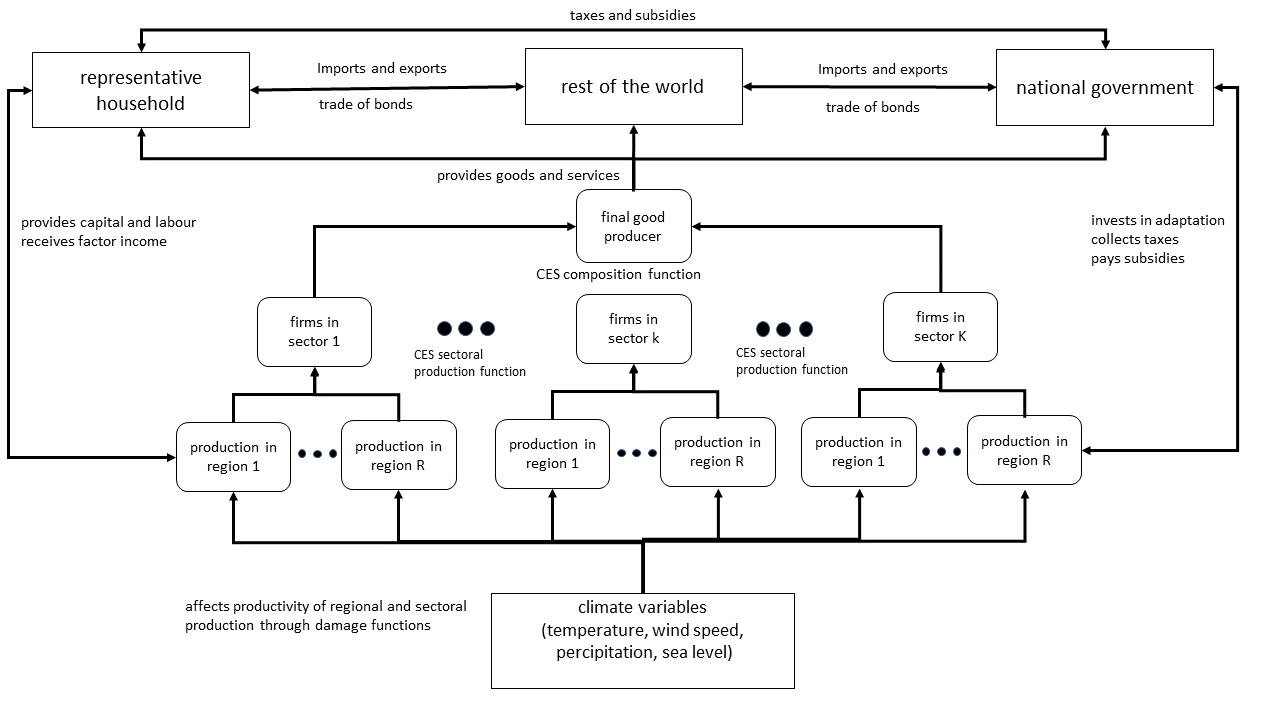
\includegraphics[width = 1\textwidth]{pictures/Model_Structure.png}
\end{frame}


\subsection{Folder Structure}
\subsubsection{Main Folder Structure}
\begin{frame}<presentation>
\frametitle{{\thesection.\thesubsection.\thesubsubsection} Main Folder Structure}
\begin{itemize}
\item The main file containing all necessary mod-files is {\tt DGE\_CRED\_Model.mod}. This file includes the following files stored in the {\tt ModFiles} folder
\item Subroutines responsible for finding the initial and terminal conditions are located in the subfolder {\tt Functions}
\item To define scenarios and structural parameters you need to create an Excel file located in the subfolder {\tt ExcelFiles}
\end{itemize}
\end{frame}

\subsubsection{Mod Files}
\begin{frame}<presentation>
\frametitle{{\thesection.\thesubsection.\thesubsubsection} Mod Files}
\begin{itemize}
\item The main file containing all necessary mod-files is {\tt DGE\_CRED\_Model.mod}. This file includes the following files stored in the {\tt ModFiles} folder:
\begin{itemize}
\item {\tt DGE\_CRED\_Model\_Declarations.mod} declares all endogenous and exogenous variables of the model and structural parameters.
\item {\tt DGE\_CRED\_Model\_Parameters.mod} assigns values to the structural parameters of the model.
\item {\tt DGE\_CRED\_Model\_Equations.mod} contains the equations of the model.
\item {\tt DGE\_CRED\_Model\_LatexOutput.mod} produces latex output for documentation of the declared variables and model equations.
\item {\tt DGE\_CRED\_Model\_SteadyState.mod} computes initial and terminal condition for the dynamic simulation.
\item {\tt DGE\_CRED\_Model\_Simulations.mod} starts the dynamic simulation.
\end{itemize}
\end{itemize}
\end{frame}

\subsubsection{Functions}
\begin{frame}<presentation>
\frametitle{{\thesection.\thesubsection.\thesubsubsection} Functions}
\begin{itemize}
%\setcounter{enumi}{1}
\item Subroutines responsible for finding the initial and terminal conditions are located in the subfolder {\tt Functions}:
\begin{itemize}
\item {\tt Calibration.mat} finds the initial conditions to reflect a specific year of the economy.
\item {\tt FindA.mat} looks for exogenous productivity shocks across sectors and regions to meet the terminal conditions.
\item {\tt FindK.mat} looks for a capital allocation across sectors and regions to fulfill the static equations of the model.
\item {\tt rng.mat} random number generator function necessary for Octave users.
\item {\tt LoadExogenous.mat} reads exogenous variables for different scenarios.
\end{itemize}
\end{itemize}
\end{frame}

\subsubsection{Excel Files}
\begin{frame}<presentation>
\frametitle{{\thesection.\thesubsection.\thesubsubsection} Excel Files}
\begin{itemize}
%\setcounter{enumi}{2}
\item To define scenarios and structural parameters you need to create an Excel file located in the subfolder {\tt ExcelFiles}:
\begin{itemize}
\item {\tt ModelSimulationandCalibrationforKSectorsandRregions.xlsx} has multiple sheets:
\begin{itemize}
\item initial {\tt Start}
\item terminal {\tt Terminal}
\item parameters to define rigidity parameters {\tt Dynamics}
\item elasticity parameters and tax rates {\tt Structural Parameters}
\item coefficients for regional and sector specific damage functions {\tt Climate Damage Functions (Labour, Capital, TFP)}
\item {\tt Baseline} scenario and other optional scenario sheets {\tt Adaptation and Extremes} defining paths for exogenous variables 
\item {\tt Data} to load external data sources
\end{itemize}
\end{itemize}
\end{itemize}
\end{frame}


\subsubsection{Mod Files}
\begin{frame}<presentation>
\frametitle{{\thesection.\thesubsection.\thesubsubsection} Mod Files}
\begin{itemize}
\item We will now define and implement all model equations into Dynare.
\item For each Equation we will explain its derivation and how to implement it.
\item The folder ModFiles contains the file \texttt{DGE\_CRED\_Model\_Equations.mod}.
\item \texttt{DGE\_CRED\_Model\_Equations.mod} contains all model equations.
\item We need to use the symbols defined in \texttt{DGE\_CRED\_Model\_Declarations.mod}.
\item Please add the missing equations in \texttt{DGE\_CRED\_Model\_Equations\_missing.mod}.
\end{itemize}
\end{frame}


\subsection{Demand}
\subsubsection{Households}
\begin{frame}
\frametitle{{\thesection.\thesubsection.\thesubsubsection} Households}
\scriptsize
\begin{itemize}
\item Representative households $h$ providing labour $N$ and capital $K$ to domestic firms $f$
\item Maximize discounted utility over an infinite horizon by choosing consumption $C_t(h)$, capital $K_{k,r,t+1}(h)$, investments $I_{k,r,t}(h)$, labour $N_{k,r,t}(h)$ and foreign net wealth $B_{t+1}$
\item Optimization problem of the representative household is
\begin{align*}
 & \underset{C_t(h), \, K_{k,r,t+1}(h), \, I_{k,r,t}(h), , \, N_{k,r,t}(h), \, B_{t+1}}{\mbox{max}} \sum_{t=0}^{\infty} \beta^{t} \left(\frac{C_{t}(h)^{1 - \sigma^{C}}}{1 - \sigma^{C}} - \sum_{k=1}^{K} \sum_{r=1}^{R} A^{N}_{k,r,t} \, \phi^{L}_{k,r} \frac{N_{k,r,t}(h)^{1+\sigma^{L}}}{1+\sigma^{L}} \right) \\
\mbox{s.t.} & P_{t} \, C_{t}(h) \, (1+\tau^{C})+\sum_{k=1}^{K} \sum_{r=1}^{R} P_{k,r,t} I_{k,r,t}(h)+B_{t+1}(h) = \\
 & \sum_{k=1}^{K} \sum_{r=1}^{R} (1 - \tau^{N}) \, W_{k,r,t} N_{k,r,t}(h)+\sum_{k=1}^{K} \sum_{r=1}^{R} P_{k,r,t} \, r_{k,r,t} \, (1 - \tau^{K}) \, K_{k,r,t}(h)+S^{f}_{t} \, \phi^{B}_{t} \, (1+r^{f}_{t} )\, B_{t}(h)
 %K_{k,r,t+1} = (1 - \delta - D^K_{k,r,t}) \, K_{k,r,t} - I_{k,r,t} \, \Gamma\left(\frac{I_{k,r,t}}{I_{k,r,t-1}}\right).
\end{align*}
\end{itemize}
\end{frame}

\subsubsection{Households Lagrangian}
\begin{frame}
\frametitle{{\thesection.\thesubsection.\thesubsubsection} Households Lagrangian}
\scriptsize
\begin{itemize}
\item We set-up the Lagrangian for the optimization problem to derive the first order conditions.
\begin{align*}
& \sum_{t=0}^{\infty} \beta^{t} \Bigg[ \left(\frac{C_{t}(h)^{1 - \sigma^{C}}}{1 - \sigma^{C}} - \sum_{k=1}^{K} \sum_{r=1}^{R} A^{N}_{k,r,t} \, \phi^{L}_{k,r} \frac{N_{k,r,t}(h)^{1+\sigma^{L}}}{1+\sigma^{L}} \right) \\
& - \lambda_{t}(h) \Big(P_{t} \, C_{t}(h) \, (1+\tau^{C})+\sum_{k=1}^{K} \sum_{r=1}^{R} P_{k,r,t} I_{k,r,t}(h)+B_{t+1}(h) - \sum_{k=1}^{K} \sum_{r=1}^{R} (1 - \tau^{N}) \, W_{k,r,t} N_{k,r,t}(h) \\
& - \sum_{k=1}^{K} \sum_{r=1}^{R} P_{k,r,t} \, r_{k,r,t} \, (1 - \tau^{K}) \, K_{k,r,t}(h) - S^{f}_{t} \, \phi^{B}_{t} \, (1+r^{f}_{t} )\, B_{t}(h) \Big) \\
& - \sum_{k=1}^{K} \sum_{r=1}^{R} \lambda_{t}(h) \omega^{I}_{k,r,t}(h) \left\lbrace K_{k,r,t+1} - (1 - \delta - D^K_{k,r,t}) \, K_{k,r,t} - I_{k,r,t} \, \Gamma\left(\frac{I_{k,r,t}}{I_{k,r,t-1}}\right) \right\rbrace\Bigg] .
\end{align*}
\end{itemize}
\end{frame}

\subsubsection{Households First Order Conditions -- Intratemporal}
\begin{frame}
\frametitle{{\thesection.\thesubsection.\thesubsubsection} Households First Order Conditions -- Intratemporal}
\scriptsize
\begin{itemize}
\item Marginal utility of consumption
\begin{align*}
\lambda_{t} =\frac{C_{t}(h)^{-\sigma^{C}}}{P_{t}\, (1+\tau^C)}
\end{align*}
\item Labour supply curve
\begin{align*}
\phi^{L}_{k,r} \, A^{N}_{k,r,t} \, N_{k,r,t}(h)^{\sigma^{L}} = \lambda_{t}(h) \, W_{k,r,t} \, (1 - \tau^{N}) \\
\end{align*}
\end{itemize}
\end{frame}

\subsubsection{Implementation of Households First Order Conditions -- Intratemporal}
\begin{frame}[fragile]
\frametitle{{\thesection.\thesubsection.\thesubsubsection} Implementation of Households First Order Conditions -- Intratemporal}

\begin{lstlisting}[frame = single]
model;
...
    @# for sec in 1:Sectors
        @# for reg in 1:Regions
        ...
        [name = 'HH FOC labour',mcp = 'N_@{sec}_@{reg}>0']
        (1 - tauN_p)*W_@{sec}_@{reg}*(P*C/PoP)^(-sigmaC_p)/(1+tauC_p) = 
        A_N_@{sec}_@{reg}*phiL_@{sec}_@{reg}_p*(N_@{sec}_@{reg})^(sigmaL_p);
        ...						
        @# endfor // end loop over regions
    @# endfor // end loop over sectors
...
end;
\end{lstlisting}
\end{frame}


\subsubsection{Households First Order Conditions -- Intertemporal}
\begin{frame}
\frametitle{{\thesection.\thesubsection.\thesubsubsection} Households First Order Conditions -- Intertemporal}
\scriptsize
\begin{itemize}
\item Euler equation for capital
\begin{align*}
\lambda_{t+1}(h) \, \beta \, \left(P_{k,r,t+1} \, r_{k,r,t+1} \, (1 - \tau^K)+(1 - \delta - D^{K}_{k,r,t+1}) \, \omega^{I}_{k,r,t+1} \right) = \lambda_{t}(h) \, \omega^{I}_{k,r,t}.
\end{align*}
\item Euler equation for investment
\begin{align*}
P_{k,r,t} \, \lambda_{t}(h) = \lambda_{t}(h) \, \omega^{I}_{k,r,t} \, \left(\Gamma(\frac{I_{k,r,t}}{I_{k,r,t-1}})+\frac{\partial \Gamma(\frac{I_{k,r,t}}{I_{k,r,t-1}})}{\partial (\frac{I_{k,r,t}}{I_{k,r,t-1}})} \, \frac{I_{k,r,t}}{I_{k,r,t-1}} \right) - \beta \lambda_{t+1}(h) \, \omega^{I}_{k,r,t+1} \, \frac{\partial \Gamma(\frac{I_{k,r,t+1}}{I_{k,r,t}})}{\partial (\frac{I_{k,r,t+1}}{I_{k,r,t}})} \, \left(\frac{I_{k,r,t+1}}{I_{k,r,t}}\right)^2
\end{align*}
\item Investment adjustment cost
\begin{align*}
\Gamma(\frac{I_{k,r,t}}{I_{k,r,t-1}}) = 3 - exp\left\lbrace\sqrt{\phi^{K}/2}\left(\frac{I_{k,r,t}}{I_{k,r,t-1}}-1\right\rbrace\right) - exp\left\lbrace-\sqrt{\phi^{K}/2}\left(\frac{I_{k,r,t}}{I_{k,r,t-1}}-1\right)\right\rbrace
\end{align*}
\end{itemize}
\end{frame}


\subsubsection{Implementation of Households First Order Conditions -- Intertemporal}
\begin{frame}[fragile]
\frametitle{{\thesection.\thesubsection.\thesubsubsection} Implementation of Households First Order Conditions -- Intertemporal (1)}

\begin{lstlisting}[frame = single]
...
# Gamma_@{sec}_@{reg} = (3 - (exp(sqrt(phiK_p/2)*(I_@{sec}_@{reg}/I_@{sec}_@{reg}(-1)-1))
                       +exp(-sqrt(phiK_p/2)*(I_@{sec}_@{reg}/I_@{sec}_@{reg}(-1)-1))));
												
# Gammapr_@{sec}_@{reg} = -I_@{sec}_@{reg}/I_@{sec}_@{reg}(-1)*sqrt(phiK_p/2)*
                          (exp(sqrt(phiK_p/2)*(I_@{sec}_@{reg}/I_@{sec}_@{reg}(-1)-1))
                          -exp(-sqrt(phiK_p/2)*(I_@{sec}_@{reg}/I_@{sec}_@{reg}(-1)-1)));
													
# Gammaprp1_@{sec}_@{reg} =  I_@{sec}_@{reg}(+1)^2/(I_@{sec}_@{reg})^2*sqrt(phiK_p/2)*
                             (exp(sqrt(phiK_p/2)*(I_@{sec}_@{reg}(+1)/I_@{sec}_@{reg}-1)) 
                             -exp(-sqrt(phiK_p/2)*(I_@{sec}_@{reg}(+1)/I_@{sec}_@{reg}-1)));
														
# Gammap1_@{sec}_@{reg} = (3 - (exp(sqrt(phiK_p/2)*(I_@{sec}_@{reg}/I_@{sec}_@{reg}(-1)-1))
                         +exp(-sqrt(phiK_p/2)*(I_@{sec}_@{reg}/I_@{sec}_@{reg}(-1)-1))));
...
\end{lstlisting}
\end{frame}

\begin{frame}[fragile]
\frametitle{{\thesection.\thesubsection.\thesubsubsection} Implementation of Households First Order Conditions -- Intertemporal (2)}

\begin{lstlisting}[frame = single]
...
[name = 'HH FOC capital',mcp = 'K_@{sec}_@{reg}>0']
(C(+1)/PoP(+1))^(-sigmaC_p)/(P(+1)*(1+tauC_p))*beta_p*r_@{sec}_@{reg}(+1)*P_@{sec}_@{reg}(+1)*(1 - tauK_p)
+ (C(+1)/PoP(+1))^(-sigmaC_p)/(P(+1)*(1+tauC_p))*omegaI_@{sec}_@{reg}(+1) 
* beta_p*(1 - delta_p - D_K_@{sec}_@{reg}(+1))
= omegaI_@{sec}_@{reg}*(C/PoP)^(-sigmaC_p)/(P*(1+tauC_p));

[name = 'HH FOC investment',mcp = 'I_@{sec}_@{reg} > 0']       
(C/PoP)^(-sigmaC_p)/(P*(1+tauC_p))*P_@{sec}_@{reg} = 
(C/PoP)^(-sigmaC_p)/(P*(1+tauC_p))*omegaI_@{sec}_@{reg}*(Gamma_@{sec}_@{reg}+Gammapr_@{sec}_@{reg})
+ beta_p*(C(+1)/PoP(+1))^(-sigmaC_p)/(P(+1)*(1+tauC_p))*omegaI_@{sec}_@{reg}(+1)*Gammaprp1_@{sec}_@{reg};
				
[name = 'LOM capital',mcp = 'I_@{sec}_@{reg} > 0']

...
\end{lstlisting}
\end{frame}

\subsubsection{Rest of the world}
\begin{frame}
\frametitle{{\thesection.\thesubsection.\thesubsubsection} Rest of the world}
\scriptsize
\begin{itemize}
\item Euler equation foreign bonds
\begin{align*}
\lambda_{t+1} \, \beta \, S^{f}_{t+1} \, \phi^{B}_{t+1} \left(1+{{r^{f}}_{t+1}}\right) = \lambda_{t}
\end{align*}
\item Effective exchange rate $S^f$ and the world interest rate $r^f$.
\item The required interest rate is above the world interest rate if the foreign debt ($B_{t+1}<0$)/ foreign claims ($B_{t+1}>0$) relative to GDP increases/decreases and future net exports relative to GDP will decrease. 
\begin{align*}
\phi^{B}_{t+1} = exp \left(-\phi^B \,(S^{f}_{t+1} \, r^{f}_{t+1} \, \frac{B_{t+1}}{Y_{t+1}}+\frac{NX_{t+1}}{Y_{t+1}})\right)
\end{align*}
\end{itemize}
\end{frame}

\subsubsection{Implementation Rest of the World}
\begin{frame}[fragile]
\frametitle{{\thesection.\thesubsection.\thesubsubsection} Implementation Rest of the World}

\begin{lstlisting}[frame = single]
...


[name = 'Foreign Assets']

...
\end{lstlisting}
\end{frame}


\subsubsection{Government Budget Constraint}
\begin{frame}
\frametitle{{\thesection.\thesubsection.\thesubsubsection} Government Budget Constraint}
\scriptsize
\begin{itemize}
\item We are interested in different policy measures taken by the government to adapt to a new climate regime. 
\item Government behaviour is not a result of an optimization problem. 
\begin{align*}
G_{t}+\sum_{k}^{K} \sum_{r}^{R} \sum_{z}^{Z} G^{A,z}_{k,r,t}+B^G_{t+1} =& \sum_{k}^{K} \sum_{r}^{R} \, \left\lbrace (\tau^{K}+\tau_{r,k,t}^{K}) \, P_{k,r,t} \, r_{k,r,t} \, K_{k,r,t}+(\tau^{N}+\tau_{k,r,t}^{N}) \, W_{k,r,t} \, N_{k,r,t} \, Pop_{t} \right\rbrace \nonumber \\
&+(1+r^{f}_{t}) \, S^{f}_{t} \phi^{B}_{t} \, B^G_{t}
\end{align*}
\end{itemize}
\end{frame}

\subsubsection{Implementation of Government Budget Constraint}
\begin{frame}[fragile]
\frametitle{{\thesection.\thesubsection.\thesubsubsection} Implementation of Government Budget Constraint}

\begin{lstlisting}[frame = single]
...
[name = 'Government Budget Constraint']
G+BG
@# for sec in 1:Sectors
 
@# endfor
= (1+rf)*Sf*exp(-phiB_p*((Sf*rf*B(-1)/Y+NX/Y)))*BG (-1)+tauC_p*C
@# for sec in 1:Sectors
    
@# endfor
;

[name = 'Government Budget Deficit']
BG = exo_BG;
...
\end{lstlisting}
\end{frame}

\subsubsection{Government Policy Instruments}
\begin{frame}
\frametitle{{\thesection.\thesubsection.\thesubsubsection} Government Policy Instruments}
\scriptsize
\begin{itemize}
\item Governments can invest into adaptation capital stocks
\begin{align*}
K^{A,z}_{k,r,t+1} = \eta^{A,z}_{k,r,t}
\end{align*}
\item Evolution of adaptation capital stocks
\begin{align*}
K^{A,z}_{k,r,t+1} = (1 - \delta_{K^{A,z},k,r}) \, K^{A,z}_{k,r,t} + G^{A,z}_{k,r,t} \nonumber \\
\end{align*}
\item Tax on capital expenditures paid by firms
\begin{align*}
\tau^{K}_{k,r,t} = \tau^{K}_{k,r,0} + \eta^{\tau^{K}}_{k,r,t} \nonumber \\
\end{align*}
\item Tax rate on wage bill paid by firms
\begin{align*}
\tau^{N}_{k,r,t} = \tau^{N}_{k,r,0} + \eta^{\tau^{N}}_{k,r,t} \nonumber \\
\end{align*}
\end{itemize}
\end{frame}

\subsubsection{Implementation of Government Policy Instruments}
\begin{frame}[fragile]
\frametitle{{\thesection.\thesubsection.\thesubsubsection} Implementation of Government Policy Instruments}

\begin{lstlisting}[frame = single]
...
@# for z in ["T", "WS", "PREC", "SL", "CYC", "DRO"]
 [name = 'sector specific adaptation expenditures by the government against sea level rise']


 [name = 'sector specific adaptation capital against sea level rise']

@# endfor
[name = 'sector specific corporate tax rate paid by firms']


[name = 'sector specific labour tax rate paid by firms']

...
\end{lstlisting}
\end{frame}

\subsubsection{Resource constraint}
\begin{frame}
\frametitle{{\thesection.\thesubsection.\thesubsubsection} Resource constraint}
\scriptsize
\begin{itemize}
\item Households and government use domestic final goods $Y_t$ produced by firms for consumption, investment and for exports $X_{t}$ and can also use imports $M_t$ for consumption and investment
\begin{align}
Y_{t} = C_{t} + I_{t} + G_{t} + \underbrace{X_{t} - M_{t}}_{NX_{t}}
\end{align}
\item The aggregation of the budget constraints of the representative households also states that positive net exports are used to increase net financial wealth to the rest of the world.
\begin{align}
NX_t = B_{t+1} - (1 + r^{f}_{t}) S^{f}_{t} \phi^B_{t} B_{t}
\end{align}
\end{itemize}
\end{frame}

\subsubsection{Implementation of Resource Constraint}
\begin{frame}[fragile]
\frametitle{{\thesection.\thesubsection.\thesubsubsection} Implementation of Resource Constraint}

\begin{lstlisting}[frame = single]
...
[name = 'Resource Constraint']
Y = C + I + G + NX
@# for sec in 1:Sectors



@# endfor
;

[name = 'Net Exports']
NX = (B - (1 + rf) * exp(-phiB_p*((Sf*rf*B(-1)/Y+NX/Y))) * Sf * B(-1));
...
\end{lstlisting}
\end{frame}
%
\subsection{Production}

\subsubsection{Sectoral Decomposition}
\begin{frame}
\frametitle{{\thesection.\thesubsection.\thesubsubsection} Sectoral Decomposition}
\scriptsize
\begin{itemize}
\item Final domestic goods $Y_{t}$ are created combining goods from different sectors $Y_{k,t}$ using a CES production function.
\begin{align}
\underset{Y_{k,t}}{\mathrm{min}} & \sum_{k} Y_{k,t} \, P_{k,t} \\ 
Y_{t} &= \left(\sum_{k} {\omega^{Q}_{k}}^{\frac{1}{\eta^Q}} Y_{k,t}^{\frac{\eta^Q-1}{\eta^Q}} \right)^{\frac{\eta^Q}{\eta^Q-1}}
\end{align}

\item Therefore, the demand for sectoral products correspond to the first order conditions of the above optimization problem. 
\begin{align*}
\frac{P_{k,t}}{P_{t}} &= {\omega^{Q}_{k}}^{\frac{1}{\eta^Q}} \left(\frac{Y_{k,t}}{Y_{t}}\right)^{\frac{-1}{\eta^Q}}
\end{align*}
\end{itemize}
\end{frame}

\subsubsection{Implementation of Sectoral Decomposition}
\begin{frame}[fragile]
\frametitle{{\thesection.\thesubsection.\thesubsubsection} Implementation of Sectoral Decomposition}
\begin{lstlisting}[frame = single]
...
[name = 'demand for sector output']

...
\end{lstlisting}

\begin{lstlisting}[frame = single]
[name = 'aggregate gross value added']
P*Y = 
@# for sec in 1:Sectors
   + P_@{sec}*Y_@{sec}
@# endfor
;
\end{lstlisting}

\end{frame}


\subsubsection{Regional Decomposition}
\begin{frame}
\frametitle{{\thesection.\thesubsection.\thesubsubsection} Regional Decomposition}
\scriptsize
\begin{itemize}
\item In order to model regional economic activity we further decompose the production process on a regional level.
\begin{align*}
\underset{Y_{k,r,t}}{\mathrm{min}} & \sum_{k} Y_{k,r,t} \, P_{k,r,t} \\ 
Y_{k,t} &= \left(\sum_{k} {\omega^{Q}_{k,r}}^{\frac{1}{\eta^Q_{k}}} Y_{k,r,t}^{\frac{\eta^Q_{k}-1}{\eta^Q_{k}}} \right)^{\frac{\eta^Q_{k}}{\eta^Q_{k}-1}}
\end{align*}
\item Demand for sectoral and regional products correspond to the first order conditions of the above optimization problem.
\begin{align*}
\frac{P_{k,r,t}}{P_{k,t}} &= {\omega^{Q}_{k,r}}^{\frac{1}{\eta^{Q}_{k}}} \left(\frac{Y_{k,r,t}}{Y_{k,t}}\right)^{\frac{-1}{\eta^{Q}_{k}}}
\end{align*}
\end{itemize}
\end{frame}

\subsubsection{Implementation of Regional Decomposition}
\begin{frame}[fragile]
\frametitle{{\thesection.\thesubsection.\thesubsubsection} Implementation of Regional Decomposition}

\begin{lstlisting}[frame = single]
...
[name = 'demand for regional sector output',mcp = 'Y_@{sec}_@{reg} > 0']
P_@{sec}_@{reg} = omegaQ_@{sec}_@{reg}_p^(1/etaQ_@{sec}_p)
                 *((Y_@{sec}_@{reg})/Y_@{sec})^(-1/etaQ_@{sec}_p)*P_@{sec};
...
\end{lstlisting}

\begin{lstlisting}[frame = single]
...
[name = 'sector aggregate specific output']



...
\end{lstlisting}
\end{frame}

\subsubsection{Regional Production}
\begin{frame}
\frametitle{{\thesection.\thesubsection.\thesubsubsection} Regional Production}
\scriptsize
\begin{itemize}
\item At the regional and sectoral level are representative firms maximizing profits using capital $K_{k,r,t}$ and labour $L_{k,r,t} = N_{k,r,t} \, Pop_{t}$ provided by households to produce products. 
\item They charge a price $P_{k,r,t}$ for their products and have to pay households wages $W_{k,r,t}$, interest on rented capital $P_{r,k,t} \, r_{r,k,t}$, taxes related to the wage bill $\tau^{N}_{r,k,t}$ and on capital expenditure $\tau^{K}_{r,k,t}$.
\item Representative firms have access to a regional and sector specific constant elasticity of substitution production function.
\item The productivity of capital and labour of a firm in one sector and region depends on the climate variables, and the adaption measures by the government represented by a damage function affecting total factor productivity $A_{k,r,t}$ by $D_{k,r,t} = D_{k,r}\left(T_{r,t}, \, PREC_{r,t}, \, WS_{r,t}, \, SL_{r,t}, \, CYC_{r,t}, \, DRO_{r,t}, \, G^{A}_{r,k,t} \right)$.
\item Further, we explicitly differentiate between climate induced damages affecting labour productivity $D_{N,k,r,t}$ and capital depreciation $D_{K,k,r,t}$. 
\item As in \cite{nordhaus1993optimal}, we assume a polynomial functional form of the damage functions, but the damages are different across regions and sectors.
\end{itemize}
\end{frame}

\subsubsection{Damages on TFP}
\begin{frame}
\frametitle{{\thesection.\thesubsection.\thesubsubsection} Damages on TFP}
\tiny
\begin{align*}
{{D_{k,r}}_{t}} &= \Big\lbrace \nonumber \\
 & (\underbrace{{{a_{T,1,k,r}}} \, {{T_{r}}_{t}}+{{a_{T,2,k,r}}}\, \left({T_{r}}_{t}\right)^{a_{T,3,k,r}}}_{\mbox{impact of temperature}})  \, \underbrace{exp(-\phi^{G^{A,T}}_{k,r} K^{A,T}_{k,r,t})}_{\mbox{impact of adaptation}} \, 
 + (\underbrace{{{a_{SL,1,k,r}}}\, {{SL}_{t}}+{{a_{SL,2,k,r}}}\, \left({SL}_{t}\right)^{{{a_{SL,3,k,r}}}}}_{\mbox{impact of sea level}})   \, \underbrace{I(SL > \frac{K^{A,SL}_{k,r,t}}{\phi^{G^{A,SL}}_{k,r}})}_{\mbox{impact of adaptation}} \\
& +  (\underbrace{{{a_{WS,1,k,r}}}\, {{WS_{r}}_{t}}+{{a_{WS,2,k,r}}}\, \left({WS_{r}}_{t}\right)^{{{a_{WS,3,k,r}}}}}_{\mbox{impact of wind speed}}) \, \underbrace{exp(-\phi^{G^{A,WS}}_{k,r} K^{A,WS}_{k,r,t})}_{\mbox{impact of adaptation}} \\
& + (\underbrace{{{a_{PREC,1,k,r}}} \, {{PREC_{r}}_{t}}+{{a_{PREC,2,k,r}}}\, \left({PREC_{r}}_{t}\right)^{{{a_{PREC,3,k,r}}}}}_{\mbox{impact of precipitation}}) \, \underbrace{exp(-\phi^{G^{A,PREC}}_{k,r} K^{A,PREC}_{k,r,t})}_{\mbox{impact of adaptation}} \nonumber \\
& +  (\underbrace{{{a_{CYC,1,k,r}}}\, {{CYC_{r}}_{t}}+{{a_{CYC,2,k,r}}}\, \left({CYC_{r}}_{t}\right)^{{{a_{CYC,3,k,r}}}}}_{\mbox{impact of cyclones}}) \, \underbrace{exp(-\phi^{G^{A,CYC}}_{k,r} K^{A,CYC}_{k,r,t})}_{\mbox{impact of adaptation}} \\
& +  (\underbrace{{{a_{DRO,1,k,r}}} \, {{DRO_{r}}_{t}}+{{a_{DRO,2,k,r}}}\, \left({DRO_{r}}_{t}\right)^{{{a_{DRO,3,k,r}}}}}_{\mbox{impact of droughts}}) \, \underbrace{exp(-\phi^{G^{A,DRO}}_{k,r} K^{A,DRO}_{k,r,t})}_{\mbox{impact of adaptation}} \\
& \Big\rbrace.
\end{align*}
\end{frame}

\subsubsection{Implementation of Damages on TFP}
\begin{frame}[fragile]
\frametitle{{\thesection.\thesubsection.\thesubsubsection} Implementation of Damages on TFP}

\begin{lstlisting}[frame = single]
...
[name = 'sector specific damage function']




...
\end{lstlisting}
\end{frame}

\subsubsection{Damages on Labour Productivity}
\begin{frame}
\frametitle{{\thesection.\thesubsection.\thesubsubsection} Damages on Labour Productivity}
\scriptsize
\begin{align*}
{{D^{N}_{k,r}}_{t}}=& \Big( \nonumber \\
&\underbrace{{{a^{N}_{T,1,k,r}}} \, {{T_{r}}_{t}}+{{a^{N}_{T,2,k,r}}}\, \left({T_{r}}_{t}\right)^{a^{N}_{T,3,k,r}}}_{\mbox{impact of temperature}} + 
\underbrace{{{a^{N}_{SL,1,k,r}}}\, {{SL}_{t}}+{{a^{N}_{SL,2,k,r}}}\, \left({SL}_{t}\right)^{{{a^{N}_{SL,3,k,r}}}}}_{\mbox{impact of sea level}} \nonumber \\
+ & \underbrace{{{a^{N}_{WS,1,k,r}}}\, {{WS_{r}}_{t}}+{{a^{N}_{WS,2,k,r}}}\, \left({WS_{r}}_{t}\right)^{{{a^{N}_{WS,3,k,r}}}}}_{\mbox{impact of wind speed}} 
+ (\underbrace{{{a^{N}_{PREC,1,k,r}}} \, {{PREC_{r}}_{t}}+{{a^{N}_{PREC,2,k,r}}}\, \left({PREC_{r}}_{t}\right)^{{{a^{N}_{PREC,3,k,r}}}}}_{\mbox{impact of precipitation}}) \,  \nonumber \\
+ & \underbrace{{{a^{N}_{CYC,1,k,r}}}\, {{CYC_{r}}_{t}}+{{a^{N}_{CYC,2,k,r}}}\, \left({CYC_{r}}_{t}\right)^{{{a^{N}_{CYC,3,k,r}}}}}_{\mbox{impact of cyclones}}
+ \underbrace{{{a^{N}_{DRO,1,k,r}}} \, {{DRO_{r}}_{t}}+{{a^{N}_{DRO,2,k,r}}}\, \left({DRO_{r}}_{t}\right)^{{{a^{N}_{DRO,3,k,r}}}}}_{\mbox{impact of droughts}} \nonumber \\
&\Big).
\end{align*}
\end{frame}

\subsubsection{Implementation of Damages on Labour Productivity}
\begin{frame}[fragile]
\frametitle{{\thesection.\thesubsection.\thesubsubsection} Implementation of Damages on Labour Productivity}

\begin{lstlisting}[frame = single]
...
[name = 'sector specific damage function on labour productivity']
D_N_@{sec}_@{reg} = min(1,aN_T_1_@{sec}_@{reg}_p * T_@{reg} + aN_T_2_@{sec}_@{reg}_p * T_@{reg}^(aN_T_3_@{sec}_@{reg}_p) + 
aN_SL_1_@{sec}_@{reg}_p * SL + aN_SL_2_@{sec}_@{reg}_p * SL^(aN_SL_3_@{sec}_@{reg}_p) +
aN_W_1_@{sec}_@{reg}_p * WS_@{reg} + aN_W_2_@{sec}_@{reg}_p * WS_@{reg}^(aN_W_3_@{sec}_@{reg}_p) + 
aN_P_1_@{sec}_@{reg}_p * PREC_@{reg} + aN_P_2_@{sec}_@{reg}_p * PREC_@{reg}^(aN_P_3_@{sec}_@{reg}_p) + 
aN_DR_1_@{sec}_@{reg}_p * DRO_@{reg} + aN_DR_2_@{sec}_@{reg}_p * DRO_@{reg}^(aN_DR_3_@{sec}_@{reg}_p) +
aN_CY_1_@{sec}_@{reg}_p * CYC_@{reg} + aN_CY_2_@{sec}_@{reg}_p * CYC_@{reg}^(aN_CY_3_@{sec}_@{reg}_p)
);
...
\end{lstlisting}
\end{frame}


\subsubsection{Damages on Capital}
\begin{frame}
\frametitle{{\thesection.\thesubsection.\thesubsubsection} Damages on Capital}
\scriptsize
\begin{align*}
{{D^{K}_{k,r}}_{t}}=& \Big( \nonumber \\
&\underbrace{{{a^{K}_{T,1,k,r}}} \, {{T_{r}}_{t}}+{{a^{K}_{T,2,k,r}}}\, \left({T_{r}}_{t}\right)^{a^{K}_{T,3,k,r}}}_{\mbox{impact of temperature}}+ \underbrace{{{a^{K}_{SL,1,k,r}}}\, {{SL}_{t}}+{{a^{K}_{SL,2,k,r}}}\, \left({SL}_{t}\right)^{{{a^{K}_{SL,3,k,r}}}}}_{\mbox{impact of sea level}} \nonumber \\
+ & \underbrace{{{a^{K}_{WS,1,k,r}}}\, {{WS_{r}}_{t}}+{{a^{K}_{WS,2,k,r}}}\, \left({WS_{r}}_{t}\right)^{{{a^{K}_{WS,3,k,r}}}}}_{\mbox{impact of wind speed}}
+ \underbrace{{{a^{K}_{PREC,1,k,r}}} \, {{PREC_{r}}_{t}}+{{a^{K}_{PREC,2,k,r}}}\, \left({PREC_{r}}_{t}\right)^{{{a^{K}_{PREC,3,k,r}}}}}_{\mbox{impact of precipitation}} \nonumber \\
+ & \underbrace{{{a^{K}_{CYC,1,k,r}}}\, {{CYC_{r}}_{t}}+{{a^{K}_{CYC,2,k,r}}}\, \left({CYC_{r}}_{t}\right)^{{{a^{K}_{CYC,3,k,r}}}}}_{\mbox{impact of cyclones}}
+ \underbrace{{{a^{K}_{DRO,1,k,r}}} \, {{DRO_{r}}_{t}}+{{a^{K}_{DRO,2,k,r}}}\, \left({DRO_{r}}_{t}\right)^{{{a^{K}_{DRO,3,k,r}}}}}_{\mbox{impact of droughts}} \nonumber \\
&\Big).
\end{align*}
\end{frame}

\subsubsection{Implementation of Damages on Capital}
\begin{frame}[fragile]
\frametitle{{\thesection.\thesubsection.\thesubsubsection} Implementation of Damages on Capital}

\begin{lstlisting}[frame = single]
...
[name = 'sector specific damage function on capital formation']
D_K_@{sec}_@{reg} = min(1,aK_T_1_@{sec}_@{reg}_p*T_@{reg}+aK_T_2_@{sec}_@{reg}_p*T_@{reg}^(aK_T_3_@{sec}_@{reg}_p)+ 
aK_SL_1_@{sec}_@{reg}_p*SL+aK_SL_2_@{sec}_@{reg}_p*SL^(aK_SL_3_@{sec}_@{reg}_p)+
aK_W_1_@{sec}_@{reg}_p*WS_@{reg}+aK_W_2_@{sec}_@{reg}_p*WS_@{reg}^(aK_W_3_@{sec}_@{reg}_p)+
aK_P_1_@{sec}_@{reg}_p*PREC_@{reg}+aK_P_2_@{sec}_@{reg}_p*PREC_@{reg}^(aK_P_3_@{sec}_@{reg}_p)+
aK_DR_1_@{sec}_@{reg}_p*DRO_@{reg}+aK_DR_2_@{sec}_@{reg}_p*DRO_@{reg}^(aK_DR_3_@{sec}_@{reg}_p)+
aK_CY_1_@{sec}_@{reg}_p*CYC_@{reg}+aK_CY_2_@{sec}_@{reg}_p*CYC_@{reg}^(aK_CY_3_@{sec}_@{reg}_p)
);
...
\end{lstlisting}
\end{frame}


\subsubsection{Profit Maximization}
\begin{frame}
\frametitle{{\thesection.\thesubsection.\thesubsubsection} Profit Maximization}
\scriptsize
\begin{itemize}
\item Firms in each region and sector have access to a constant elasticity of substitution production function with production factors labour and capital.

\begin{align*}
\underset{Y_{k,r,t}, N_{k,r,t}, K_{k,r,t}}{\mathrm{max}} P_{k,r,t} \, Y_{k,r,t} - W_{k,r,t} \, N_{k,r,t} \, Pop_{t} \, (1 + \tau^{N}_{k,r,t}) - r_{k,r,t} \, P_{k,r,t} \, K_{k,r,t} \, (1 + \tau^{K}_{k,r,t})\nonumber \\ 
\mbox{s.t.} \, Y_{k,r,t} = A_{k,r,t} (1 - D_{k,r,t}) \, \left[{\alpha^{N}_{k,r}}^{\frac{1}{\eta^{NK}_{k,r}}} \, \left( A^{N}_{k,r,t} \, (1 - D^{N}_{k,r,t}) \, Pop_{t} \, N_{k,r,t}\right)^{\rho_{k,r}} + {\alpha^{K}_{k,r}}^{\frac{1}{\eta^{NK}_{k,r}}} \, \left(K_{k,r,t}\right)^{\rho_{k,r}}\right]^{\frac{1}{\rho_{k,r}}}, \nonumber \\
\mbox{ where } \rho_{k,r} = \frac{\eta^{NK}_{k} - 1}{\eta^{NK}_{k}}.
\end{align*}
\end{itemize}
\end{frame}

\subsubsection{Factor Demand}
\begin{frame}
\frametitle{{\thesection.\thesubsection.\thesubsubsection} Factor Demand}
\scriptsize
\begin{itemize}
\item Demand for production factors are given by the first order condition of the above optimization problem. The Lagrange multiplier is equal to the price charged by companies. 
\begin{align*}
\frac{W_{k,r,t}}{P_{k,r,t}}  \, (1 + \tau^{N}_{k,r,t}) = {\alpha^{N}_{k,r}}^{\frac{1}{\eta^{NK}_{k,r}}} \, \left(A_{k,r,t} \, (1 - D_{k,r,t}) \, A^N_{k,r,t} \, (1 - D^N_{k,r,t})\right)^{\rho_{k,r}} \left(\frac{Pop_{t} N_{k,r,t}}{Y_{k,r,t}}\right)^{-\frac{1}{\eta^{NK}_{k,r}}} \nonumber \\ 
r_{k,r,t} \, (1 + \tau^{K}_{k,r,t}) = {\alpha^{K}_{k,r}}^{\frac{1}{\eta^{NK}_{k,r}}} \, \left(A_{k,r,t} \, (1 - D_{k,r,t})\right)^{\rho_{k,r}}\left(\frac{K_{k,r,t}}{Y_{k,r,t}} \right)^{-\frac{1}{\eta^{NK}_{k,r}}} \\ 
\end{align*}
\item We use the more general case of the CES production function rather than the more commonly used Cobb-Douglas production function. 
\item The parameter $\eta^{NK}_{k,r}$ allows us to control the response of capital and labour demand to temporary productivity shocks. 
\item Temporary productivity shocks are in our set-up also weather extremes. 
\end{itemize}
\end{frame}

\subsubsection{Implementation of Factor Demand}
\begin{frame}[fragile]
\frametitle{{\thesection.\thesubsection.\thesubsubsection} Implementation of Factor Demand}

\begin{lstlisting}[frame = single]
...
[name='sector specific output']


[name = 'Firms FOC capital',mcp = 'K_@{sec}_@{reg} > 0']


[name = 'Firms FOC labour',mcp = 'N_@{sec}_@{reg} > 0']

...
\end{lstlisting}
\end{frame}


\subsubsection{Trade with the Rest of the World}
\begin{frame}
\frametitle{{\thesection.\thesubsection.\thesubsubsection} Trade with the Rest of the World}
\scriptsize
\begin{itemize}
\item The demand for domestic exports and foreign imports is not explicitly modeled in this version of the model. 
\item We assume that net exports follow an auto-regressive process of order one and that the long-run value of net exports depend on the long-run development of gross domestic product.
\begin{align*}
NX_{t} = \rho^{NX} \, NX_{t-1} + (1 - \rho^{NX}) \omega^{NX} P_{t} \, Y_{t} \, exp\left({{\eta_{NX}}_{t}}\right)
\end{align*}
\item The effective exchange rate $S^f_{t}$ and the world interest rate $r^{f}_{t}$ determine how much governments and households have to pay back in domestic currency as net lender or how much they receive as net borrower to the rest of the world.
 \item The world interest rate is independent of domestic developments and only the effective exchange rate adjusts.
\end{itemize}
\end{frame}

\subsubsection{Implementation of Trade with Rest of the World}
\begin{frame}[fragile]
\frametitle{{\thesection.\thesubsection.\thesubsubsection} Implementation of Trade with Rest of the World}

\begin{lstlisting}[frame = single]
...
[name = 'LOM Net Exports']
NX = rhoNX_p * NX(-1) + (1 - rhoNX_p) * exp(exo_NX) * omegaNX_p * Y * P;

[name = 'World interest rate']
rf = (1/beta_p-1);
...
\end{lstlisting}
\end{frame}

\subsection{Climate Variables}

\subsubsection{Climate Variables}
\begin{frame}
\frametitle{{\thesection.\thesubsection.\thesubsubsection} Climate Variables}
\scriptsize
\begin{itemize}
\item Average annual regional temperature is given by:
\begin{align*}
T_{r,t} = T_{r,0} + \eta^{T}_{t}
\end{align*}
\item Average annual regional wind speed is given by:
\begin{align*}
WS_{r,t} = WS_{r,0} + \eta^{WS}_{t}
\end{align*}
\item Average annual regional precipitation is given by:
\begin{align*}
PREC_{r,t} = PREC_{r,0} + \eta^{PREC}_{t}
\end{align*}

\item Sea level:
\begin{align*}
SL_{t} = SL_{0} + \eta^{SL}_{t}
\end{align*}
\end{itemize}
\end{frame}

\subsubsection{Implementation of Climate Variables}
\begin{frame}[fragile]
\frametitle{{\thesection.\thesubsection.\thesubsubsection} Implementation of Climate Variables}

\begin{lstlisting}[frame = single]
...
[name = 'Temperature']
T_@{reg} = T0_@{reg}_p + exo_T_@{reg};

[name = 'Wind speed']
WS_@{reg} = WS0_@{reg}_p + exo_WS_@{reg};

[name = 'Precipitation']
PREC_@{reg} = PREC0_@{reg}_p + exo_PREC_@{reg};

[name = 'Sea Level']
SL = SL0_p + exo_SL;
...
\end{lstlisting}
\end{frame}

\subsubsection{Weather Extremes}
\begin{frame}
\frametitle{{\thesection.\thesubsection.\thesubsubsection} Weather Extremes}
\scriptsize
\begin{itemize}
\item A score reflecting the intensity and number of annual droughts in the region.
\begin{align*}
DRO_{r,t} = DRO_{r,0} + \eta^{DRO}_{t}
\end{align*}
\item A score reflecting the intensity and number of annual cyclones in the region.
\begin{align*}
CYC_{r,t} = CYC_{r,0} + \eta^{CYC}_{t}
\end{align*}
\end{itemize}
\end{frame}

\subsubsection{Implementation of Weather Extremes}
\begin{frame}[fragile]
\frametitle{{\thesection.\thesubsection.\thesubsubsection} Implementation of Weather Extremes}

\begin{lstlisting}[frame = single]
...
[name = 'Drought']
DRO_@{reg} = DRO0_@{reg}_p + exo_DRO_@{reg};

[name = 'Cyclones']
CYC_@{reg} = CYC0_@{reg}_p + exo_CYC_@{reg};
...
\end{lstlisting}
\end{frame}

\subsection{Aggregation and Identities}

\subsubsection{National Aggregates}
\begin{frame}
\frametitle{{\thesection.\thesubsection.\thesubsubsection} National Aggregates}
\scriptsize
\begin{itemize}
\item National aggregate investment is given by:
\begin{align*}
P_{t} \, I_{t} = \sum_{k}^{K} P_{k,t} \, I_{k,t}
\end{align*}
\item National aggregate capital stock is given by:
\begin{align*}
P_{t} \, K_{t} = \sum_{k}^{K} P_{k,t} \, K_{k,t-1}
\end{align*}
\item National aggregate labour input:
\begin{align*}
N_{t} = \sum_{k}^{K} N_{k,t}
\end{align*}

\end{itemize}
\end{frame}

\subsubsection{Implementation of National Aggregates}
\begin{frame}[fragile]
\frametitle{{\thesection.\thesubsection.\thesubsubsection} Implementation of National Aggregates}

\begin{lstlisting}[frame = single]
...
[name = 'aggregate investment']
P * I = 
@# for sec in 1:Sectors
 + P_@{sec} * I_@{sec}
@# endfor
;

[name = 'aggregate capital']
P * K = 
@# for sec in 1:Sectors
 + P_@{sec} * K_@{sec}(-1)
@# endfor
;

[name = 'aggregate labour']
N = 
@# for sec in 1:Sectors
    + N_@{sec}
@# endfor
;
...
\end{lstlisting}
\end{frame}

\subsubsection{Sectoral Aggregates}
\begin{frame}
\frametitle{{\thesection.\thesubsection.\thesubsubsection} Sectoral Aggregates}
\scriptsize
\begin{itemize}
\item Sector aggregate investment is given by:
\begin{align*}
P_{k,t} \, I_{k,t} = \sum_{r}^{R} P_{k,r,t} \, I_{k,r,t}
\end{align*}
\item Sector aggregate capital stock is given by:
\begin{align*}
P_{k,t} \, K_{k,t} = \sum_{r}^{R} P_{k,r,t} \, K_{k,r,t-1}
\end{align*}
\item Sector aggregate wage bill:
\begin{align*}
W_{k,t} N_{k,t} = \sum_{r}^{R}  W_{k,r,t} N_{k,r,t}
\end{align*}
\item Sector aggregate labour input:
\begin{align*}
N_{k,t} = \sum_{r}^{R} N_{k,r,t}
\end{align*}
\end{itemize}
\end{frame}

\subsubsection{Implementation of Sectoral Aggregates}
\begin{frame}[fragile]
\frametitle{{\thesection.\thesubsection.\thesubsubsection} Implementation of Sectoral Aggregates (1)}

\begin{lstlisting}[frame = single]
...
[name = 'aggergate sector labour']
N_@{sec} = 
@# for reg in 1:Regions
+ N_@{sec}_@{reg}
@# endfor
;
[name = 'aggergate sector labour income']
W_@{sec} * N_@{sec} = 
@# for reg in 1:Regions
+ W_@{sec}_@{reg} * N_@{sec}_@{reg}
@# endfor
;
...
\end{lstlisting}
\end{frame}

\subsubsection{Implementation of Sectoral Aggregates}
\begin{frame}[fragile]
\frametitle{{\thesection.\thesubsection.\thesubsubsection} Implementation of Sectoral Aggregates (2)}

\begin{lstlisting}[frame = single]
...
[name = 'aggregate sector investment']
P_@{sec} * I_@{sec} = 
@# for reg in 1:Regions
+ P_@{sec}_@{reg} * I_@{sec}_@{reg}
@# endfor
;
[name = 'aggregate capital']
P_@{sec} * K_@{sec} = 
@# for reg in 1:Regions
+ P_@{sec}_@{reg} * K_@{sec}_@{reg}
@#
;
...
\end{lstlisting}
\end{frame}



\subsubsection{National Aggregates}
\begin{frame}
\frametitle{{\thesection.\thesubsection.\thesubsubsection} National Aggregates}
\scriptsize
\begin{itemize}
\item Sector aggregate investment is given by:
\begin{align*}
P_{k,t} \, I_{k,t} = \sum_{r}^{R} P_{k,r,t} \, I_{k,r,t}
\end{align*}
\item Sector aggregate capital stock is given by:
\begin{align*}
P_{k,t} \, K_{k,t} = \sum_{r}^{R} P_{k,r,t} \, K_{k,r,t-1}
\end{align*}
\item Sector aggregate wage bill:
\begin{align*}
W_{k,t} N_{k,t} = \sum_{r}^{R}  W_{k,r,t} N_{k,r,t}
\end{align*}
\item Sector aggregate labour input:
\begin{align*}
N_{k,t} = \sum_{r}^{R} N_{k,r,t}
\end{align*}
\end{itemize}
\end{frame}

\subsubsection{Implementation of Sectoral Aggregates}
\begin{frame}[fragile]
\frametitle{{\thesection.\thesubsection.\thesubsubsection} Implementation of Sectoral Aggregates}

\begin{lstlisting}[frame = single]
...
[name = 'aggergate sector labour']
N_@{sec} = 
@# for reg in 1:Regions
+ N_@{sec}_@{reg}
@# endfor
;
[name = 'aggergate sector labour income']
W_@{sec} * N_@{sec} = 
@# for reg in 1:Regions
+ W_@{sec}_@{reg} * N_@{sec}_@{reg}
@# endfor
;
[name = 'aggregate sector investment']
P_@{sec} * I_@{sec} = 
@# for reg in 1:Regions
+ P_@{sec}_@{reg} * I_@{sec}_@{reg}
@# endfor
;
[name = 'aggregate capital']
P_@{sec} * K_@{sec} = 
@# for reg in 1:Regions
+ P_@{sec}_@{reg} * K_@{sec}_@{reg}
@#
;
...
\end{lstlisting}
\end{frame}

\subsubsection{Population and Price Level}
\begin{frame}
\frametitle{{\thesection.\thesubsection.\thesubsubsection} Population and Price Level}
\scriptsize
\begin{itemize}
\item Population is independent of other variables in the model and is given by:
\begin{align*}
pop_{t} = pop_{0,t} + \eta^{pop}_{t}
\end{align*}
\item National price level is given by:
\begin{align*}
P_{t} = P_{0,t} + \eta^{P}_{t}
\end{align*}
\end{itemize}
\end{frame}

\subsubsection{Implementation of Population and Prices}
\begin{frame}[fragile]
\frametitle{{\thesection.\thesubsection.\thesubsubsection} Implementation of Population and Prices}

\begin{lstlisting}[frame = single]
...
[name = 'national price level']
P = P0_p * exp(exo_P);

[name = 'Population']
PoP = PoP0_p + exo_PoP;
...
\end{lstlisting}
\end{frame}




\section{Model Simulation and Calibration}
\subsection{Definitions}
\begin{frame}
\frametitle{{\thesection.\thesubsection} Main model file  \texttt{DGE\_CRED\_Model.mod}}
%\scriptsize
\begin{itemize}
\item Define number of sectors and regions 
%\begin{verbatim}
%		   ...\\
%		   @# define Sectors = 3\\
%			 @# define Regions = 3\\
%			 ...\\
%		\end{verbatim}
\item Define number of steps in steady state calculation and simulation process  
%\begin{verbatim}
	%	   ...
		%   options_.iStepSteadyState = 10;
			% options_.iStepSimulation = 20;
			 %...
		%\end{verbatim}
\item Define excel files that include:
	\begin{itemize}
		\item Data used for calibration
		\item Explicit parameter values for parameters
		\item Assumption related to scenarios
		\item Results 
	\end{itemize}
\item Declare additional  \texttt{.mod} files needed for simulation and documentation of results   
\end{itemize}
\end{frame}

\begin{frame}
\frametitle{{\thesection.\thesubsection} Definition of Sectors and Regions}
%\scriptsize
\begin{itemize}
\item Number of sectors: 3 or 9
	\begin{itemize}
		\item Agriculture, industry, services
		\item Agriculture, manufacturing, construction, transportation and storage, accommodation and food service activities, further production activities, services, state-related sectors and other service activities
	\end{itemize}	
\item Number of regions: 2, 3 or 6
	\begin{itemize}
		\item Coastal (Red River Delta, North Central and Central Coast, Southeast, Mekong river delta) and non-coastal regions
		\item Red River Delta, Mekong river delta and remaining
		\item All six individually
	\end{itemize}	
\end{itemize}
\end{frame}

\subsection{Calibration}
\subsubsection{Calibration of Parameters}
\begin{frame}
\frametitle{{\thesection.\thesubsection.\thesubsubsection} Calibration of Parameters}
%\scriptsize
\begin{itemize}
\item Regional and sectoral shares of GDP, employment and wages calibrated to match actual data
\item Assumptions about a baseline trajectory of the Vietnamese economy (without climate change effects)
	\begin{itemize}
		\item Projections for population dynamics
		\item Long-term growth projections, reflecting general economic catch-up process
		\item Speed and scale of structural change (transition to service economy)
\end{itemize}
\item Calibration of structural parameters unaffected by long-term growth and/or climate change
\end{itemize}
\end{frame}

\subsubsection{Calibration of Damage Function Parameters}
\begin{frame}
\frametitle{{\thesection.\thesubsection.\thesubsubsection} Calibration of Damage Function Parameters}
%\scriptsize
\begin{itemize}
\item Distinct damage functions for every region-sector combination 
\item Consideration of six climate change phenomena:
	\begin{itemize}
		\item Temperature $(T)$
		\item Wind Speed $(W)$
		\item Percipitation $(P)$
		\item Sea Level $(SL)$
		\item Drought $(DR)$
		\item Cyclone $(CY)$
	\end{itemize}
\item Each damage function includes parameters measuring 
	\begin{itemize}
		\item Loss of labour productivity 
		\item Depreciation of capital
		\item Loss of TFP
	\end{itemize}
w.r.t. to each of the six climate change phenomena
\end{itemize}
\end{frame}

\subsubsection{Notation of Damage Function Parameters}
\begin{frame}[fragile]
\frametitle{{\thesection.\thesubsection.\thesubsubsection} Notation of Damage Function Parameters}
%\scriptsize
\begin{itemize}
\item Damage function parameters have the general form:
\begin{verbatim}
	f\_c\_d\_s\_r\_p
\end{verbatim}
\begin{itemize}
\item Input Factor (\texttt{f}): \texttt{aN}- labour, \texttt{aK} - capital, \texttt{a} - TFP
\item Climate change phenomenon (\texttt{c}): \texttt{T} - temperature, \texttt{W} - wind speed, \texttt{P} - percipitation, \texttt{SL} - sea level, \texttt{DR} - drought, \texttt{CY} - cyclone
\item Degree of polynomial (\texttt{d}): \texttt{1} - linear, \texttt{2} - quadratic, \texttt{3} - quadratic exponent
\item Sector (\texttt{s}): \texttt{1} - agriculture, \texttt{2} - industry, \texttt{3} - services
\item Region (\texttt{r}): \texttt{1} - region 1, \texttt{2} - region 2, \texttt{3} - region 3
\end{itemize}
\end{itemize}
\end{frame}

\subsection{Scenario Analyses}
\subsubsection{Temperature}
\begin{frame}
\frametitle{{\thesection.\thesubsection.\thesubsubsection} Scenario 1 -- "`Temperature"' (1)}
\begin{itemize}
\item Assumes that average temperature increases by X degrees in a given region until the year 2100
\item Three regions example (Thuc et al, 2016):
	\begin{itemize}
		\item Mekong river delta: +4.4 degrees
		\item Red river delta: +5.4 degrees
		\item Other regions 3: +5.0 degrees
	\end{itemize}
 \item Linear increases in average temperature every year until final value is reached
\end{itemize}
\end{frame}

\begin{frame}
\frametitle{{\thesection.\thesubsection.\thesubsubsection} Scenario 1 -- "`Temperature"' (2)}
\begin{figure}
			\centering
			\subfigure{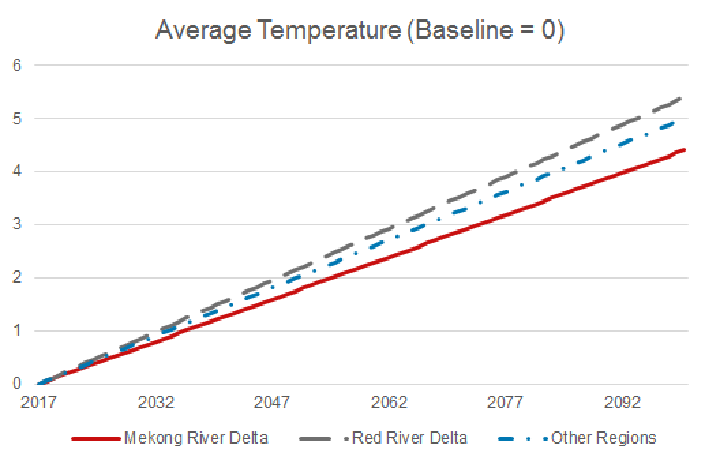
\includegraphics[width=10cm]{pictures/scenario_temperature}}\\
			\footnotesize{Source: DGE--CRED model}
		\end{figure}
\end{frame}

\begin{frame}
\frametitle{{\thesection.\thesubsection.\thesubsubsection} Scenario 1 -- "`Temperature"' (3)}
\begin{itemize}
\item Damage functions are calibrated to match results of relevant meta studies
\item Challinor et al. (2014):
	\begin{itemize}
		\item Crop yields on average decrease by 4.5\% in response to a 1 degree increase in temperature
		\item Parameter that governs loss in production from temperature increases (\texttt{a\_T\_1\_1\_r\_p}) is set to 0.045 for all regions
		\item Can be set differently for different kinds of crop or, more generally, different regions (to reflect region-specific cultivation)
	\end{itemize}
\end{itemize}
\end{frame}

\subsubsection{Sea Level}
\begin{frame}
\frametitle{{\thesection.\thesubsection.\thesubsubsection} Scenario 2 -- "`Sea Level"' (1)}
\begin{itemize}
\item Increase in average temperature as defined in scenario 1
\item In addition, assumes that the sea level rises by 100 cm until the year 2100 
\item Percentage of agricultural land at risk of inundation following a sea level rise by 100 cm (Thuc et al, 2016)
	\begin{itemize}
		\item Mekong river delta: 39\%
		\item Red river delta: 16\%
		\item Other regions: 2\%
	\end{itemize}
\end{itemize}
\end{frame}

\begin{frame}
\frametitle{{\thesection.\thesubsection.\thesubsubsection} Scenario 2 -- "`Sea Level"' (2)}
\begin{itemize}
\item Damage functions are calibrated to match percentage of agricultural land at risk of inundation
\item Different calibration for different regions
	\begin{itemize}
		\item Mekong river delta: \texttt{a\_SL\_1\_1\_1\_p} set to 0.39
		\item Red river delta: \texttt{a\_SL\_1\_1\_2\_p} set to 0.16
		\item Other regions: \texttt{a\_SL\_1\_1\_3\_p} set to 0.02
	\end{itemize}
	\item Effects of sea level rise on other sectors of production not yet included
	\item Can be extended e.g. to transportation (flooded/destroyed roads), energy etc.
\end{itemize}
\end{frame}

\subsubsection{Adaption}
\begin{frame}
\frametitle{{\thesection.\thesubsection.\thesubsubsection} Scenario 3 -- "`Adaptation"' (1)}
\begin{itemize}
\item Increase in average temperature and sea level as defined in scenario 2 
\item In addition: government measures to reduce damage from (sea level rise), e.g. dike construction. Damage functions are calibrated to match percentage of agricultural land at risk of inundation
\item Facts and assumptions
	\begin{itemize}
		\item Coast line of Mekong River Delta is 600 km
		\item Dike needs to be of the same height along the entire coastline
		\item Estimated costs: 40,000 EUR for one meter height and one meter length 
		\item Height increases with sea level each year
		\item Damages associated with sea level rise in Mekong Delta River are zero, if and only if the height of the dike exceeds the sea level rise
	\end{itemize}
\item Benefit calculated as difference in GDP between a scenario with dike (Adaptation) and without dike (Sea Level) relative to the Baseline 
\end{itemize}
\end{frame}

\begin{frame}
\frametitle{{\thesection.\thesubsection.\thesubsubsection} Scenario 3 -- "`Adaptation"' (2)}
\begin{figure}
			\centering
			\subfigure{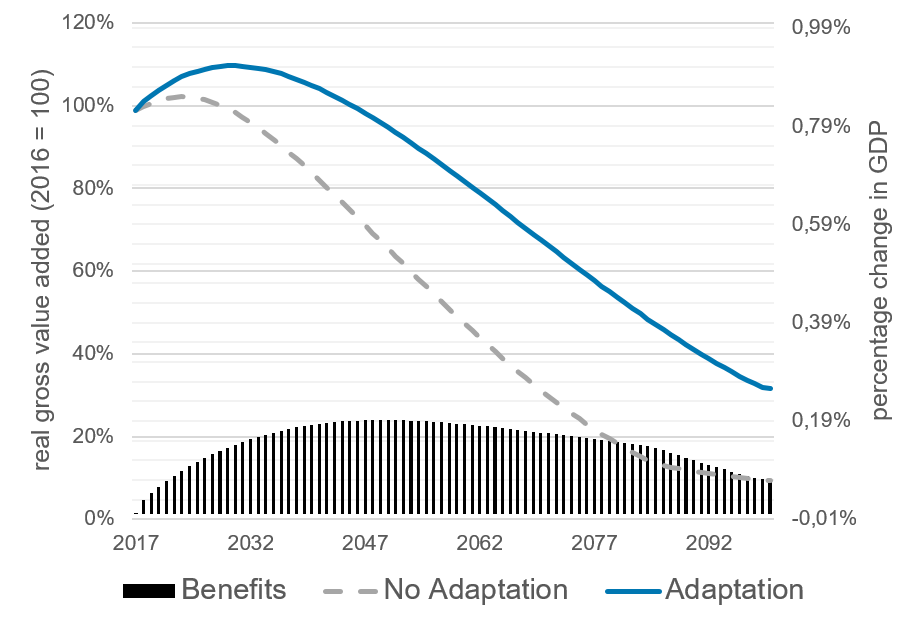
\includegraphics[width=10cm]{pictures/scenario_adaptation.png}}\\
			\footnotesize{Source: DGE--CRED model}
		\end{figure}
\end{frame}

\subsubsection{Extremes}
\begin{frame}
\frametitle{{\thesection.\thesubsection.\thesubsubsection} Scenario 4 -- "`Extremes"'}
\begin{itemize}
	\item Increase in average temperature and sea level as defined in scenario 2
	\item In addition: occurrence of cyclones and droughts 
	\item Occurrence of cyclones and droughts as well as their intensity is modeled as a random process		
\end{itemize}
\end{frame}

\subsubsection{Simulation Results}
\begin{frame}
\frametitle{{\thesection.\thesubsection.\thesubsubsection} Simulation Results}
\begin{itemize}
\item Stored in Excel file 
\item Include 
	\begin{itemize}
		\item Paths for all model variables, stored to individual sheets for every scenario
		\item Figures comparing the outcomes of different simulated scenarios
		\end{itemize}
\end{itemize}
\end{frame}

\begin{frame}<presentation>
	\centering \huge{References}
\end{frame}

\begin{frame}[allowframebreaks]%in case more than 1 slide needed
\frametitle{References}
\scriptsize{
\printbibliography}
\end{frame}

\section*{Appendix}
\begin{frame}<presentation>
	\centering \huge{Appendix}
\end{frame}
\begin{frame}<presentation>[fragile]
	\frametitle{Appendix: Illustration of the Newton Method}
	\begin{itemize}
		\item Graphical illustration of the Newton method (unidimensional):
		\begin{center}
			\begin{overlayarea}{8cm}{5.5cm}
				\only<1>{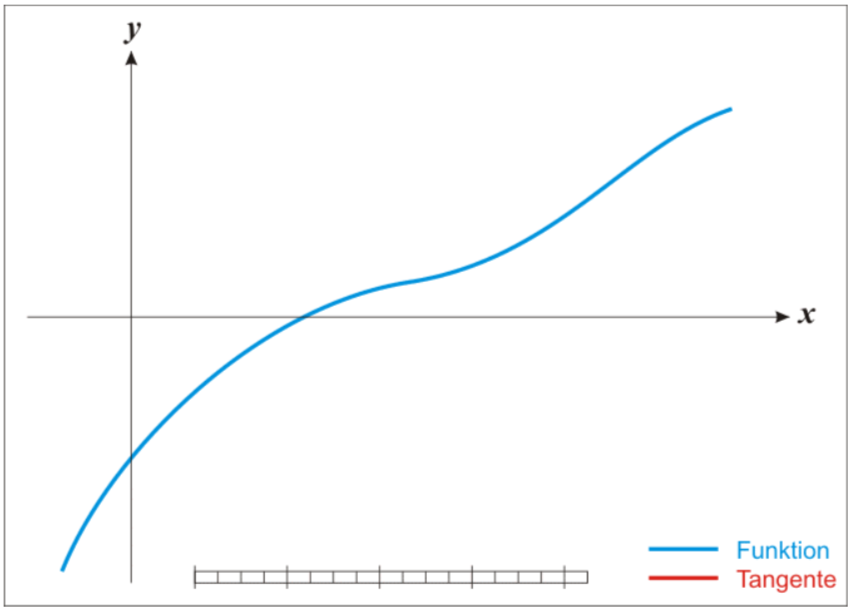
\includegraphics[width=8cm,height=5.5cm]{pictures/Newton/Newton1}}
				\only<2>{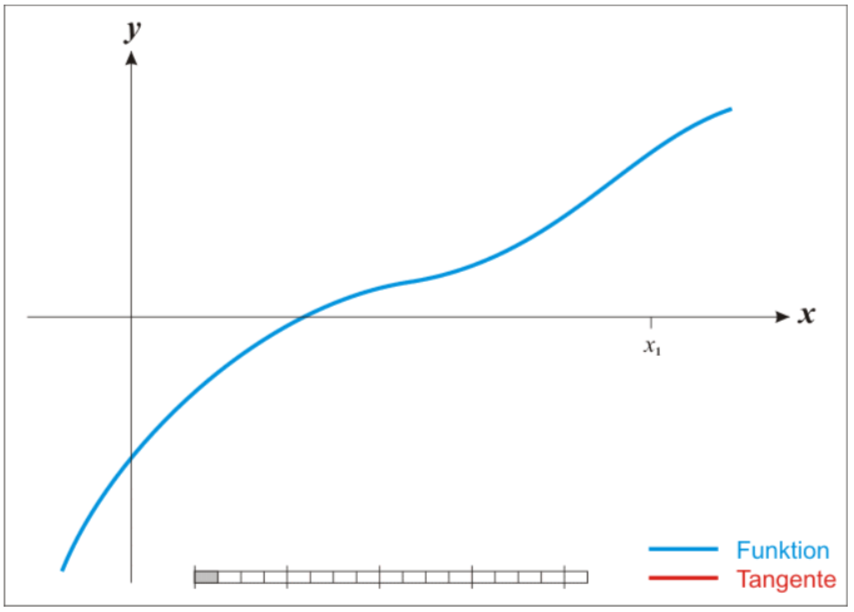
\includegraphics[width=8cm,height=5.5cm]{pictures/Newton/Newton2}}
				\only<3>{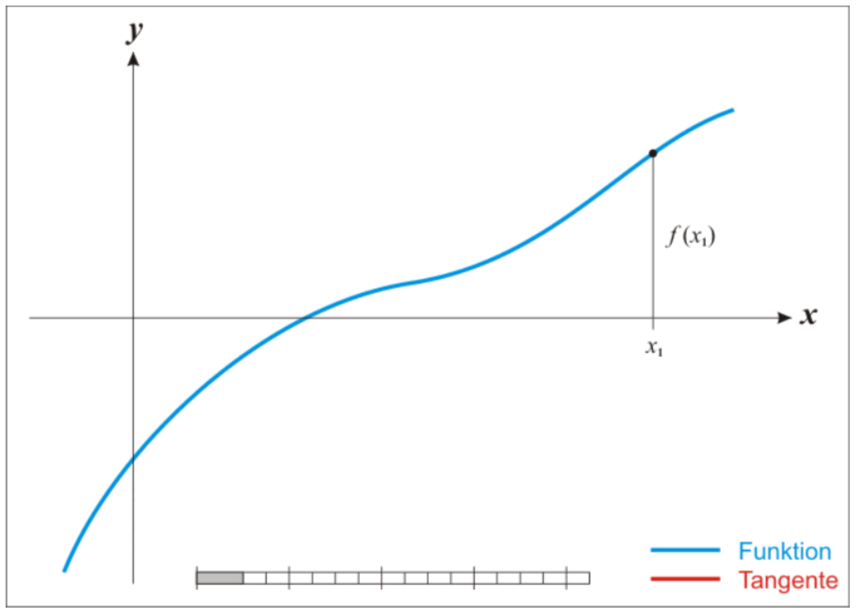
\includegraphics[width=8cm,height=5.5cm]{pictures/Newton/Newton3}}
				\only<4>{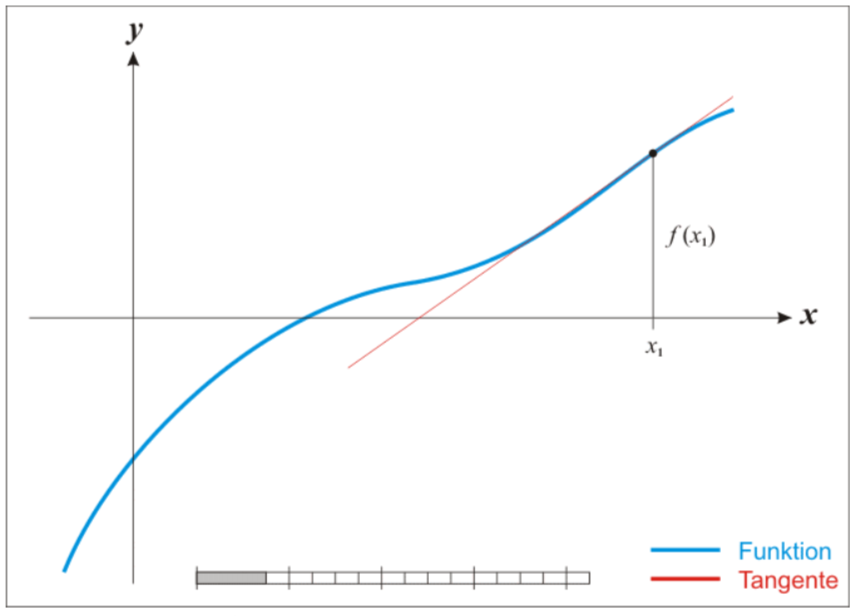
\includegraphics[width=8cm,height=5.5cm]{pictures/Newton/Newton4}}
				\only<5>{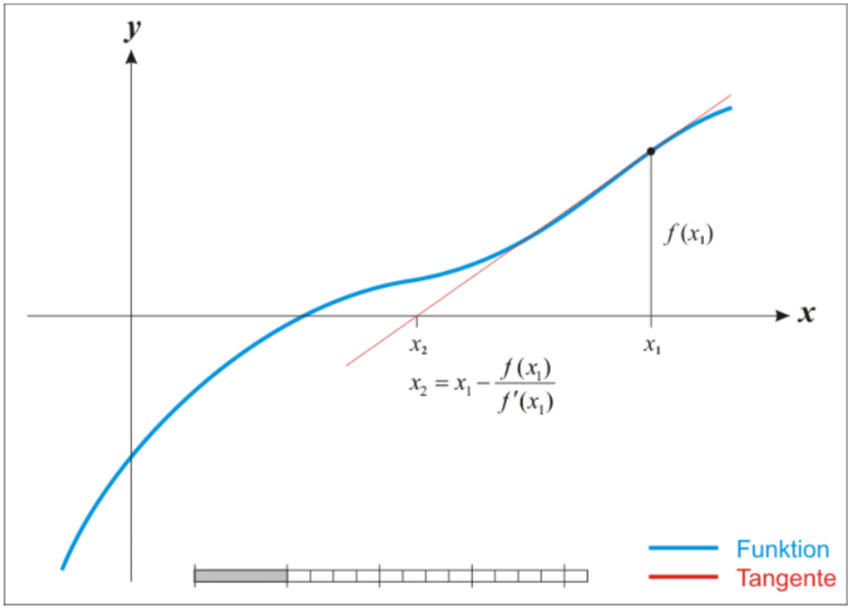
\includegraphics[width=8cm,height=5.5cm]{pictures/Newton/Newton5}}
				\only<6>{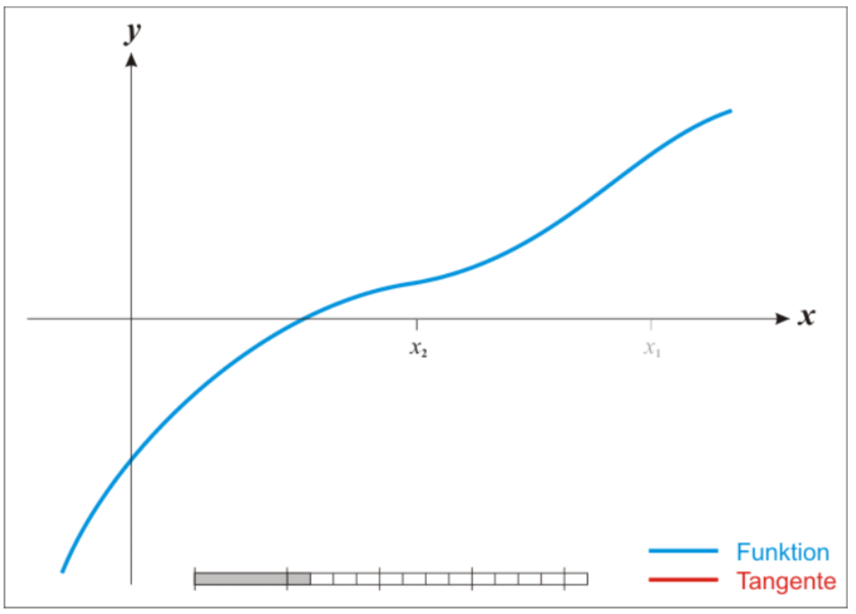
\includegraphics[width=8cm,height=5.5cm]{pictures/Newton/Newton6}}
				\only<7>{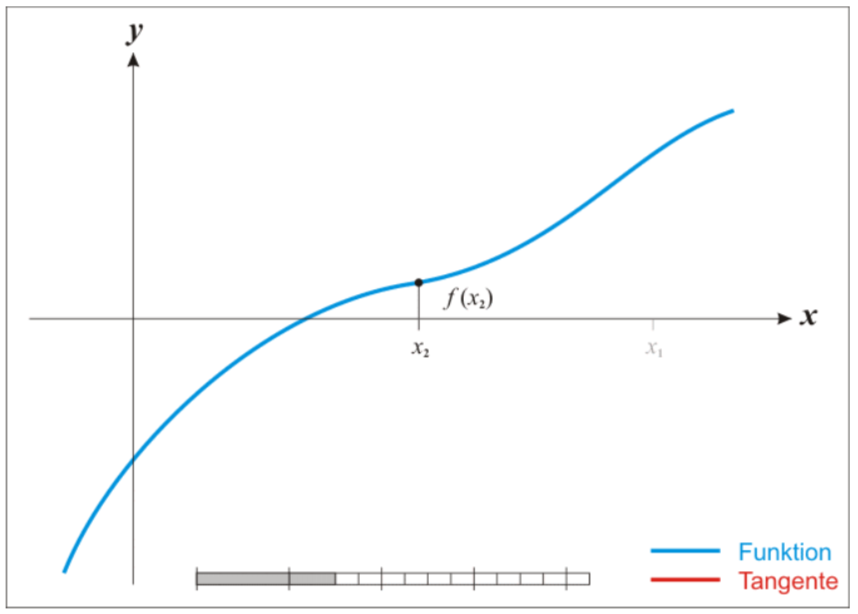
\includegraphics[width=8cm,height=5.5cm]{pictures/Newton/Newton7}}
				\only<8>{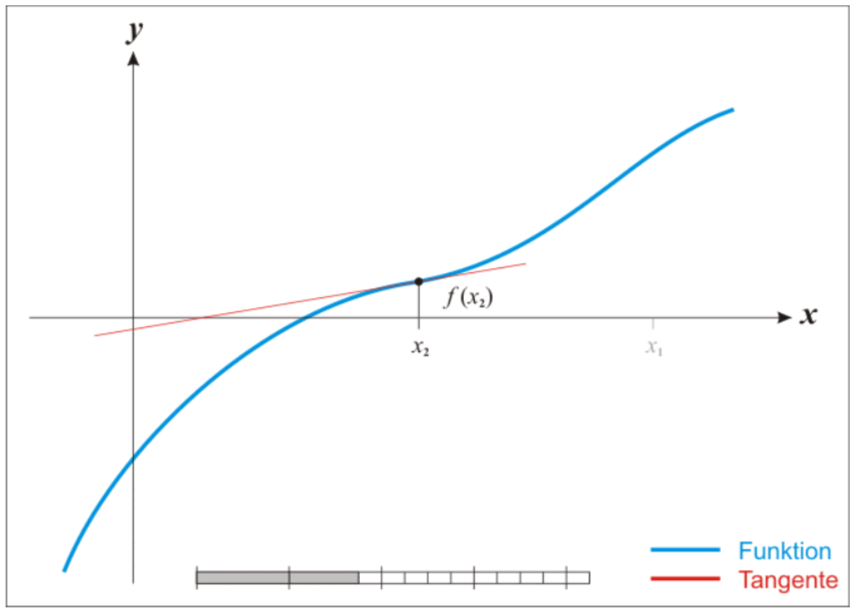
\includegraphics[width=8cm,height=5.5cm]{pictures/Newton/Newton8}}
				\only<9>{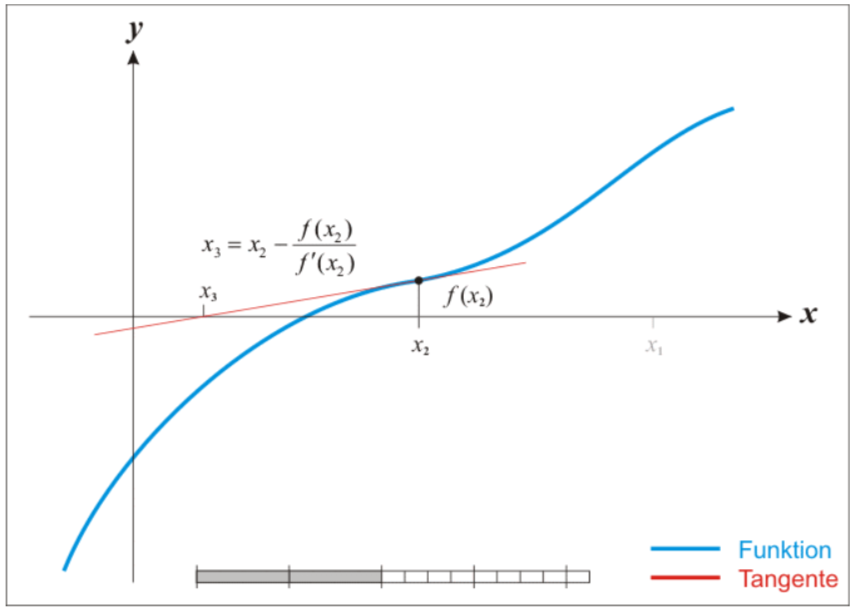
\includegraphics[width=8cm,height=5.5cm]{pictures/Newton/Newton9}}
				\only<10>{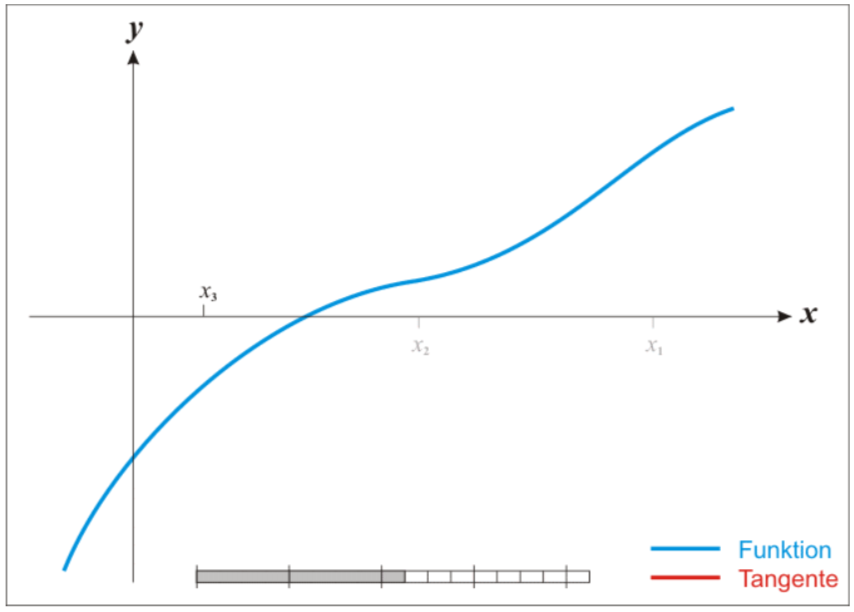
\includegraphics[width=8cm,height=5.5cm]{pictures/Newton/Newton10}}
				\only<11>{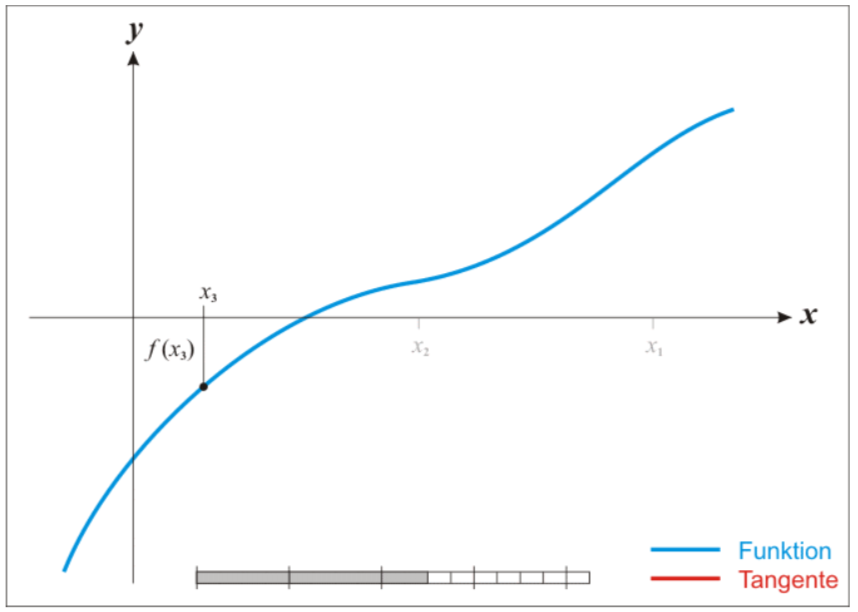
\includegraphics[width=8cm,height=5.5cm]{pictures/Newton/Newton11}}
				\only<12>{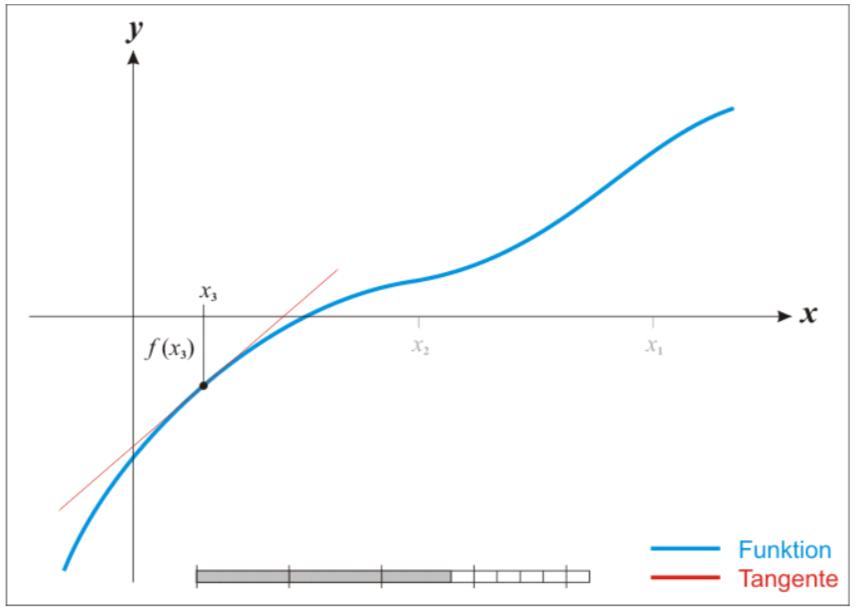
\includegraphics[width=8cm,height=5.5cm]{pictures/Newton/Newton12}}
				\only<13>{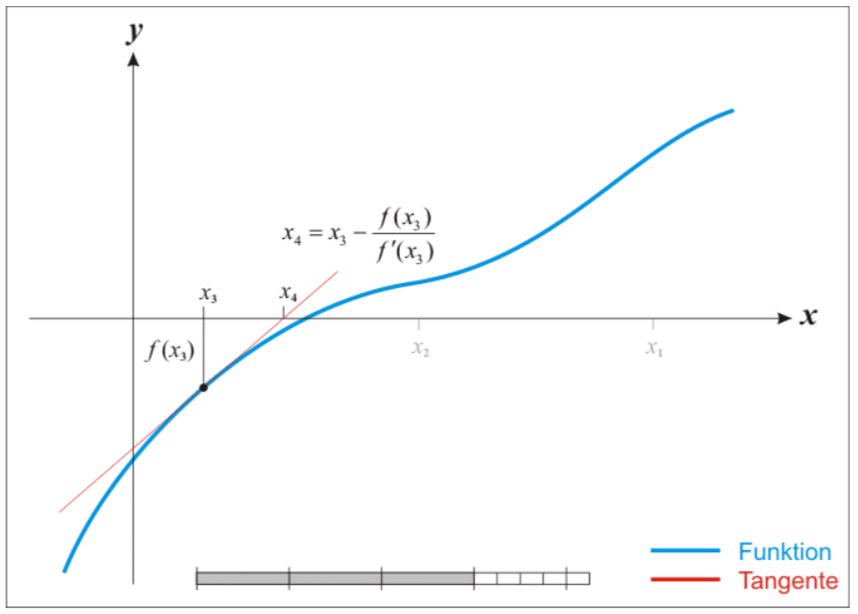
\includegraphics[width=8cm,height=5.5cm]{pictures/Newton/Newton13}}
				\only<14>{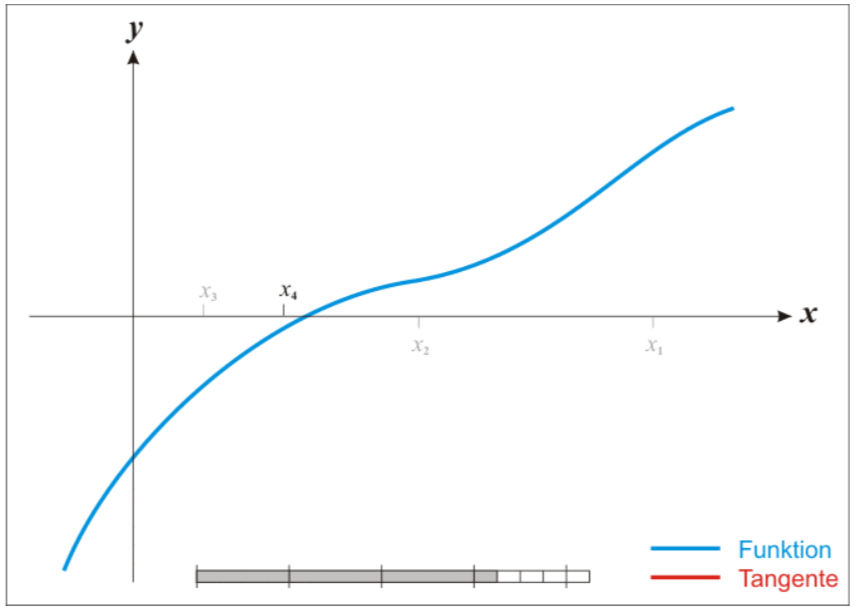
\includegraphics[width=8cm,height=5.5cm]{pictures/Newton/Newton14}}
				\only<15>{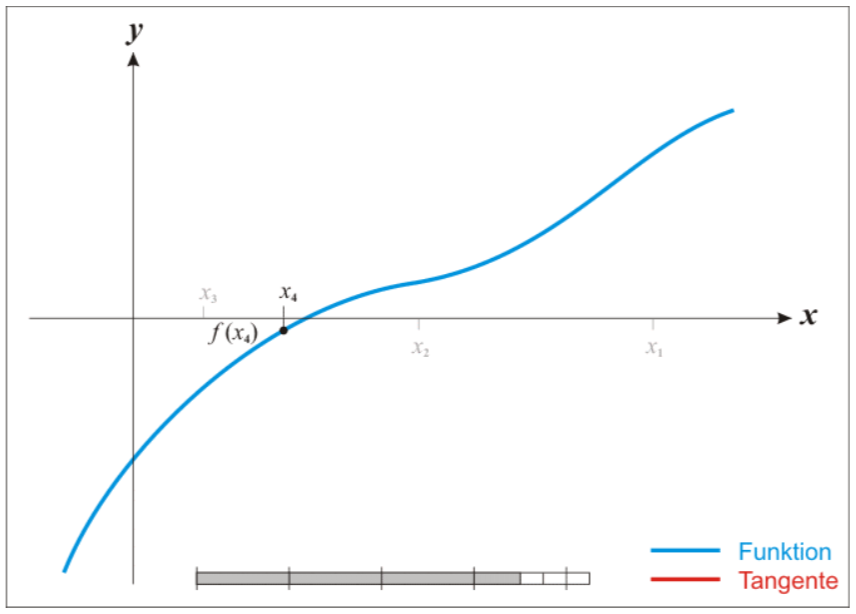
\includegraphics[width=8cm,height=5.5cm]{pictures/Newton/Newton15}}
				\only<16>{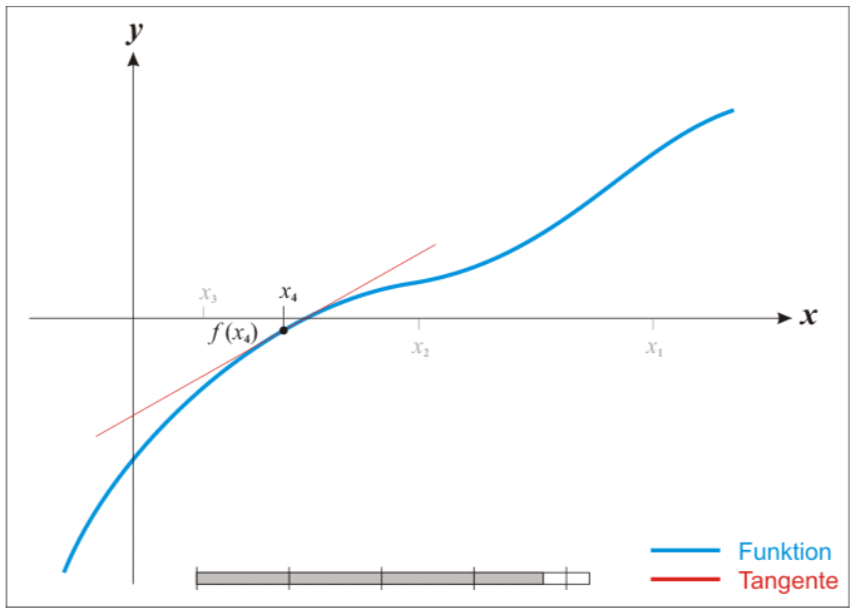
\includegraphics[width=8cm,height=5.5cm]{pictures/Newton/Newton16}}
				\only<17>{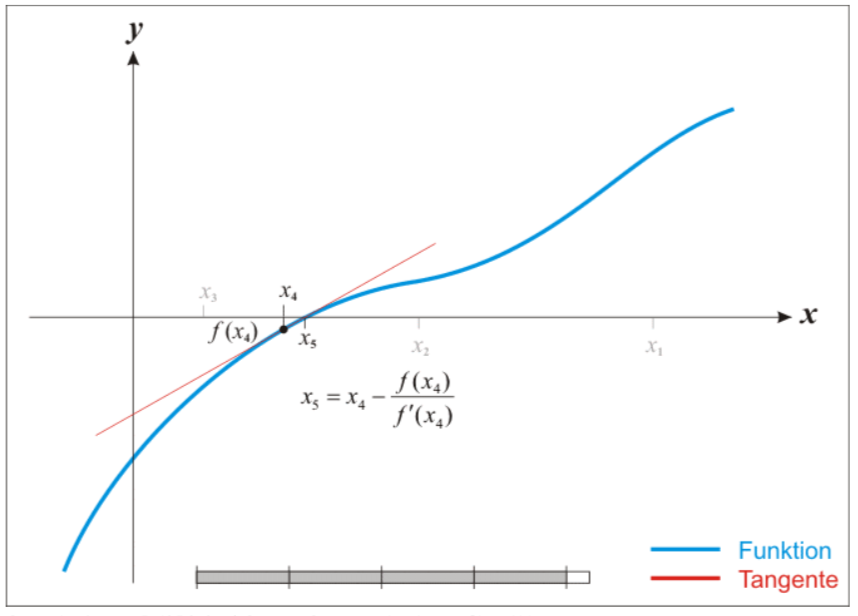
\includegraphics[width=8cm,height=5.5cm]{pictures/Newton/Newton17}}
				\only<18>{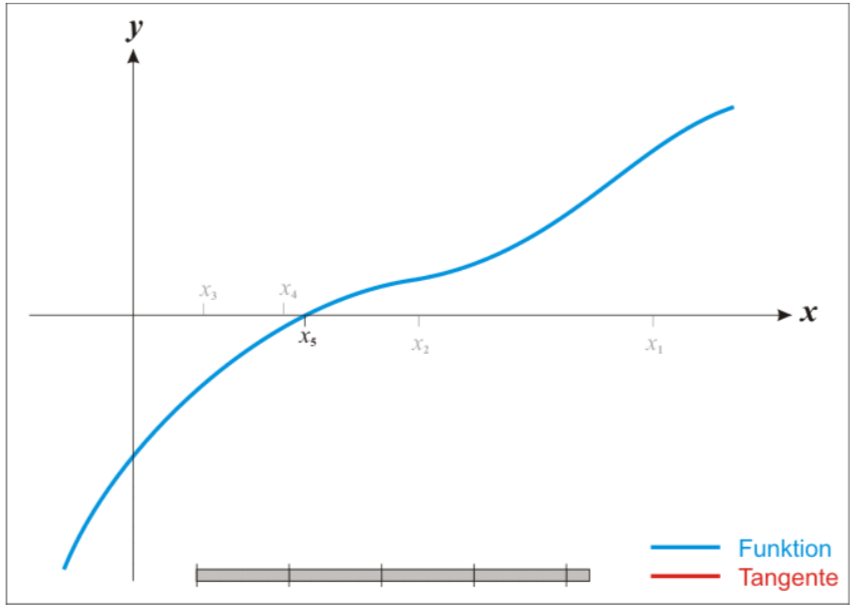
\includegraphics[width=8cm,height=5.5cm]{pictures/Newton/Newton18}}
			\end{overlayarea}
			\hspace{-1cm} \tiny{Copyright \textcopyright \enspace 2005 Ralf Pfeifer / Creative Commons Attribution-ShareAlike 3.0}
		\end{center}
	\end{itemize}
\end{frame}

\end{document}
